\documentclass[a4paper]{article}

% Basic packages
\usepackage{fontspec}
\XeTeXlinebreaklocale "zh"    % 启用中文断行（XeTeX 内建，无需 xeCJK）
\XeTeXlinebreakskip = 0pt plus 1pt
\setmainfont{Songti SC}
\setsansfont{Heiti SC}
\setmonofont{Menlo}
\usepackage{amsmath, amssymb}
\usepackage{graphicx}
\usepackage[margin=2.5cm]{geometry}
\usepackage[most]{tcolorbox}
\usepackage{etoolbox}
\usepackage{listings}
\usepackage{hyperref}
\usepackage{booktabs}
\usepackage{subcaption}
\usepackage{float}

% Chinese font setup (macOS system fonts, no ctex needed)
\setmainfont{Songti SC}
\setsansfont{Heiti SC}
\setmonofont{Menlo}
\newcommand{\song}{\fontspec{Songti SC}}
\newcommand{\hei}{\fontspec{Heiti SC}}
\newcommand{\kai}{\fontspec{KaiTi}}
\newcommand{\fangsong}{\fontspec{FangSong}}

% ===== Highlight boxes =====
\newtcolorbox{knowledgebox}[1]{
    enhanced, colback=blue!5!white, colframe=blue!75!black, colbacktitle=blue!75!black,
    coltitle=white, fonttitle=\bfseries, title=#1, attach boxed title to top left={yshift=-2mm, xshift=2mm},
    boxrule=1pt, sharp corners
}

\newtcolorbox{importantbox}[1]{
    enhanced, colback=yellow!10!white, colframe=yellow!80!black, colbacktitle=yellow!80!black,
    coltitle=black, fonttitle=\bfseries, title=#1, sharp corners
}

\newtcolorbox{warningbox}[1]{
    enhanced, colback=red!5!white, colframe=red!75!black, colbacktitle=red!75!black,
    coltitle=white, fonttitle=\bfseries, title=#1, sharp corners
}

\newtcolorbox{practicebox}[1]{
    enhanced, colback=green!5!white, colframe=green!60!black, colbacktitle=green!60!black,
    coltitle=white, fonttitle=\bfseries, title=#1, sharp corners
}

% ===== Code listings =====
\lstset{
    basicstyle=\ttfamily\small,
    keywordstyle=\color{blue},
    stringstyle=\color{red!60!black},
    commentstyle=\color{green!60!black},
    breaklines=true,
    frame=single,
    numbers=left,
    numberstyle=\tiny\color{gray},
    captionpos=b,
    extendedchars=false
}

% ===== Front-page metadata =====
\newcommand{\notetitle}{CS336 Lecture 9：Scaling Laws 1（Scaling Laws 基础）}
\newcommand{\notesubtitle}{Stanford CS336: Language Modeling from Scratch (Spring 2025)}
\newcommand{\noteauthors}{讲师：Percy Liang, Tatsu Hashimoto \quad 笔记：ZCode}
\newcommand{\notedate}{2026-07-14}
\newcommand{\videochannel}{Stanford CS336}
\newcommand{\videopublishdate}{2025 Spring}
\newcommand{\videoduration}{65 分钟}
\newcommand{\videourl}{https://www.youtube.com/watch?v=6Q-ESEmDf4Q}
\newcommand{\videocoverpath}{cover.jpg}

\begin{document}

% ===== Title page =====
\begin{titlepage}
\centering
{\Large 课程笔记\par}
\vspace{1.2cm}
{\huge\bfseries \notetitle\par}
\vspace{0.3cm}
{\large \notesubtitle\par}
\vspace{0.5cm}
{\large \noteauthors\par}
\vspace{0.3cm}
{\large \notedate\par}
\vspace{1.0cm}

\includegraphics[width=0.82\textwidth,height=0.40\textheight,keepaspectratio]{\videocoverpath}\par

\vfill
\begin{tcolorbox}[width=0.9\textwidth, colback=black!2!white, colframe=black!60, sharp corners]
\textbf{视频作者/频道}：\videochannel\par
\textbf{发布日期}：\videopublishdate\par
\textbf{视频时长}：\videoduration\par
\textbf{视频链接}：\href{\videourl}{\nolinkurl{\videourl}}
\end{tcolorbox}
\end{titlepage}

\tableofcontents
\newpage

%% --- 正文内容开始 ---

\section{本讲定位：Scaling Laws 是什么、为什么重要}

本讲是 CS336 系列"数据与扩展（Data and Scaling）"主题的开篇。前几讲讨论了 Transformer 架构、训练数据准备和 tokenizer 设计，本讲开始回答一个更具策略性的问题：\textbf{在固定 compute 预算下，应当如何分配参数、数据和训练步数}？

\subsection{核心问题}

当我们决定训练一个语言模型时，面对的是一连串相互制约的选择：

\begin{itemize}
\item 模型应该多大（参数 $N$）？
\item 数据应该多少（token 数 $D$）？
\item batch size 多大、训多少步（总 compute $C$）？
\item 学习率、optimizer、深度宽度比如何选？
\end{itemize}

这些问题如果仅靠经验或反复试错，在 billion/trillion 参数规模下成本会爆炸。\textbf{Scaling law}（扩展律）的核心想法是：先用小规模实验拟合出 loss 关于 $N$、$D$、$C$ 的解析关系，再用这个关系\emph{外推}大规模决策。

\begin{knowledgebox}{Scaling Law 的工作定义}
Scaling law 指\textbf{模型某个性能指标（通常用 loss / cross-entropy / perplexity）随规模变量（参数量 $N$、数据量 $D$、计算量 $C$）呈现的幂律（power law）关系}。在 log-log 坐标下表现为近似直线，便于外推。
\end{knowledgebox}

\subsection{为什么 scaling law 是"工程驱动"的研究范式}

Percy 在本讲开头强调：scaling law 不仅仅是经验观察，更是\textbf{工业界做大型模型训练的决策基础设施}。它直接决定了：

\begin{enumerate}
\item 一次 trillion 级训练前，需要多少小规模实验来标定超参；
\item "再多花钱"带来的边际收益能否预测；
\item compute 预算在参数和数据之间应如何切分（这正是 \textbf{Chinchilla} 论文的核心贡献）。
\end{enumerate}

\begin{figure}[H]
\centering
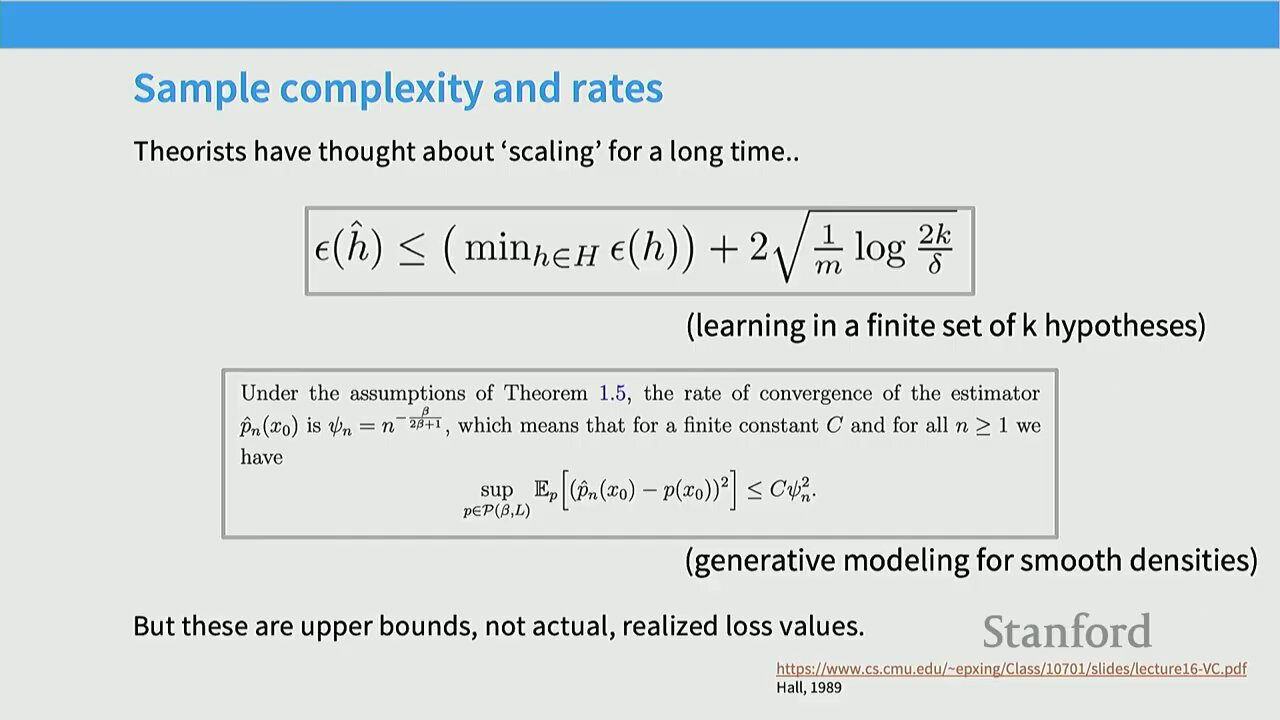
\includegraphics[width=0.92\textwidth]{figures/fig_complexity_rates.jpg}
\caption{统计学习理论给出的泛化误差界：在有限假设集下，excess risk 以 $O(1/\sqrt{m})$ 衰减。这是"理论上"的 scaling law 起点。\protect\footnotemark}
\end{figure}
\footnotetext{视频画面时间区间：00:04:00--00:04:30。}

理论给出的衰减速率 $O(1/\sqrt{m})$ 对应 log-log 斜率 $-0.5$，但\textbf{实测的衰减速率远慢于此}——这是整个 scaling law 文献的关键观察，下文将反复出现。

\section{Scaling Law 的历史脉络}

Scaling law 不是 2020 年 Kaplan 论文凭空冒出来的。Percy 用相当篇幅梳理了它的历史脉络，强调这是一个\textbf{跨越三十多年、跨多个 ML 子领域反复出现}的实证规律。

\subsection{Bell Labs 1993：最早的 scaling law 论文}

\begin{figure}[H]
\centering
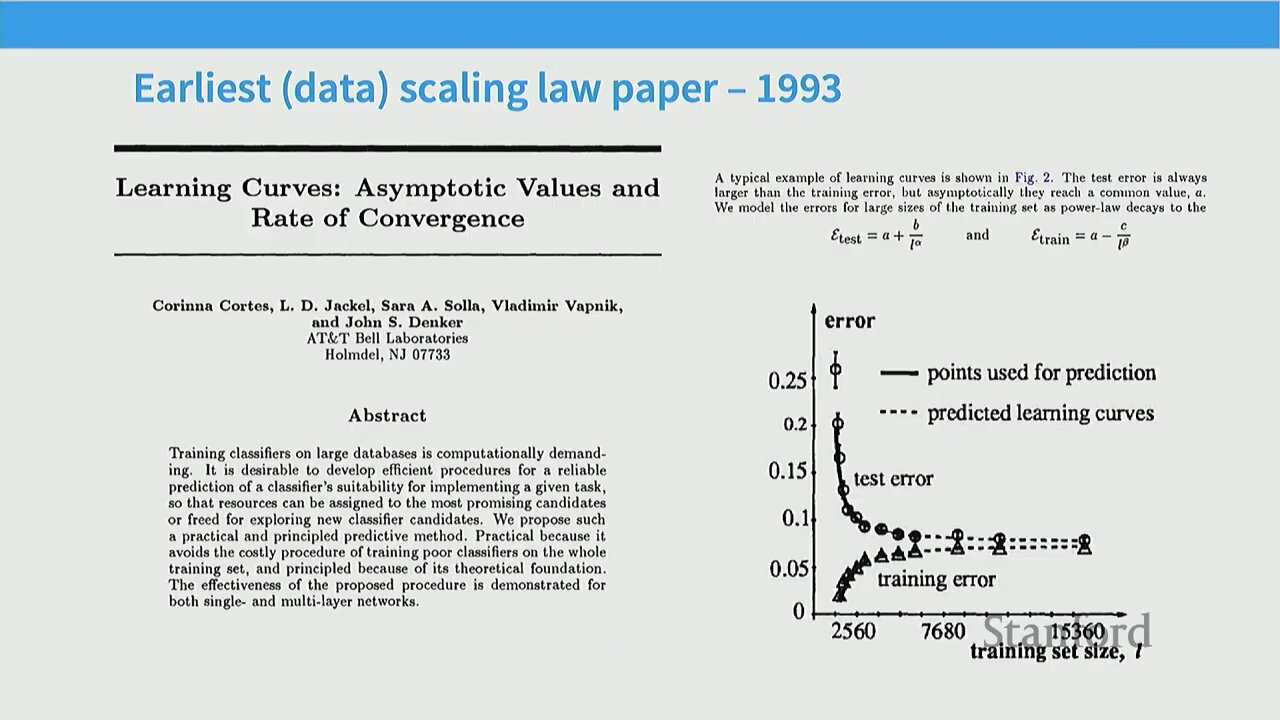
\includegraphics[width=0.92\textwidth]{figures/fig_bell_labs_1993.jpg}
\caption{Bell Labs 1993 NeurIPS 论文：在 SVM / hand-crafted 特征年代，就已观察到 test error 关于样本量呈幂律衰减，并拟合出 test error $=$ 不可约误差 $+$ 多项式衰减项 的函数形式。\protect\footnotemark}
\end{figure}
\footnotetext{视频画面时间区间：00:05:15--00:05:45。}

\begin{importantbox}{Bell Labs 函数形式}
该论文给出的形式与今天的 Chinchilla 几乎同构：
\[
L(m) \;=\; \alpha \;+\; \beta\, m^{-p}
\]
其中 $\alpha$ 是\textbf{不可约误差（irreducible error）}，$\beta\, m^{-p}$ 是\textbf{可约误差（reducible error）}，$m$ 是样本量，$p>0$ 是衰减指数。这套"两项相加"的模板沿用了三十多年。
\end{importantbox}

更值得注意的是，当年这套工具就被用来做\textbf{预测模型性能而无需完整训练}——与今天用 scaling law 决定 trillion 参数模型训练预算的逻辑完全一致。

\subsection{Banko \& Brill 2001：NLP 中的早期证据}

\begin{figure}[H]
\centering
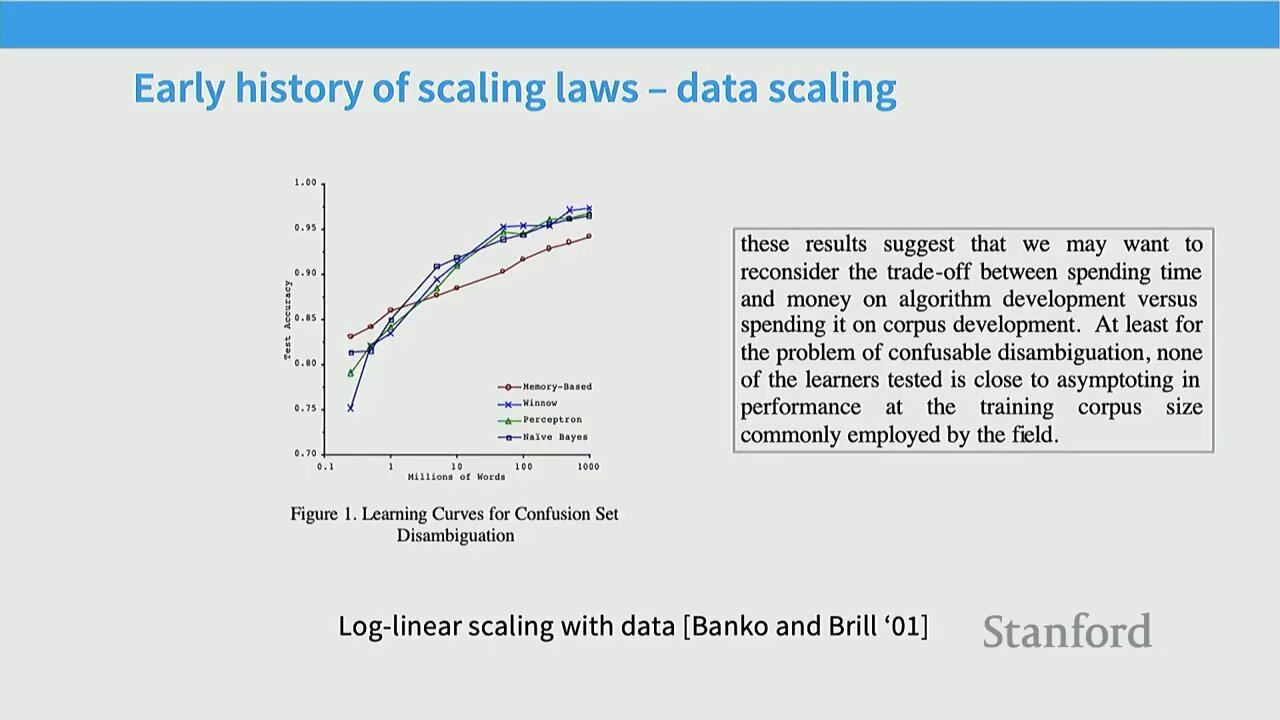
\includegraphics[width=0.92\textwidth]{figures/fig_banko_brill.jpg}
\caption{Banko \& Brill 2001：在 NLP 任务上明确观察到"算法差异在足够数据面前变得不重要"的"more data beats better algorithms"现象。\protect\footnotemark}
\end{figure}
\footnotetext{视频画面时间区间：00:07:00--00:07:30。}

Banko \& Brill 在 2001 年就发现：\textbf{在 log-log 坐标下，NLP 系统性能随数据量呈近似线性的幂律提升}，而且不同复杂度的算法最终都收敛到相近的曲线上。这预示了后来"算法选择不如数据规模"的工程直觉。

\begin{warningbox}{"算法 vs 数据"是一个工程权衡题}
Banko \& Brill 提出的取舍问题到今天仍成立：\textbf{在固定成本下，是该投入算法创新还是数据收集}？现代的答案是 scaling law 让你能定量回答——只在曲线斜率不再给收益时才转向算法创新。
\end{warningbox}

\subsection{Hestness 2017：三区域与跨任务普适性}

\begin{figure}[H]
\centering
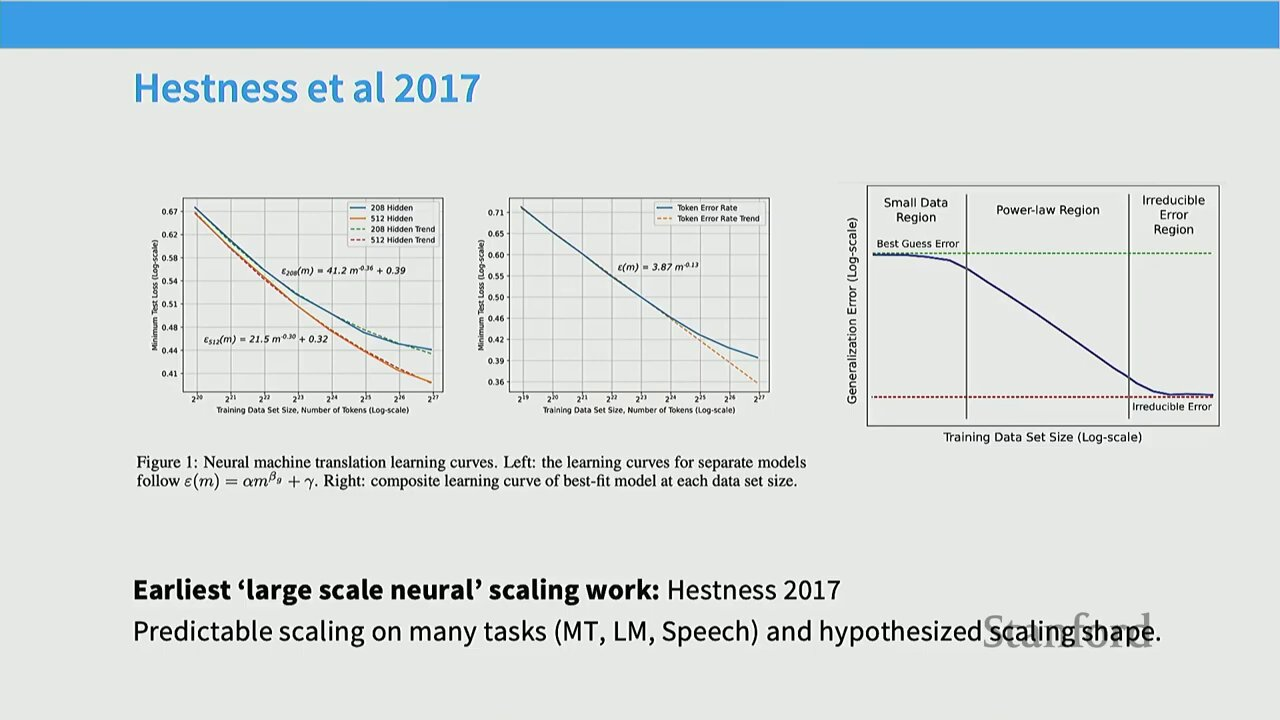
\includegraphics[width=0.92\textwidth]{figures/fig_hestness_regions.jpg}
\caption{Hestness et al.\ 2017 提出的"三区域"模型：性能随数据量变化呈现 (1) 随机猜测区、(2) 幂律缩放区、(3) 不可约误差渐近区。\protect\footnotemark}
\end{figure}
\footnotetext{视频画面时间区间：00:08:15--00:08:45。}

Hestness 在 2017 年系统性地把这一规律扩展到多个领域，并明确划分了三段：

\begin{enumerate}
\item \textbf{随机猜测区}（small data）：模型还没"学到"任何信号，性能接近随机；
\item \textbf{幂律缩放区}（power-law region）：性能随数据/规模呈幂律提升，这是 scaling law 工作的核心区域；
\item \textbf{不可约误差渐近区}（irreducible error）：曲线趋于水平，剩余误差无法通过更多数据消除。
\end{enumerate}

\begin{knowledgebox}{实测衰减指数远比理论慢}
Hestness 给出的跨任务实测指数：
\[
\begin{array}{lcl}
\text{Machine Translation} &:& p \approx 0.07 \text{--} 0.13 \\
\text{Speech Recognition} &:& p \approx 0.3 \\
\text{Language Modeling} &:& p \approx 0.95
\end{array}
\]
这些值远小于 PAC 学习理论给出的 $0.5$，说明真实任务的"难度"远超简单函数拟合。
\end{knowledgebox}

\subsection{Kaplan 2020：把 scaling law 引入 LLM 时代}

\begin{figure}[H]
\centering
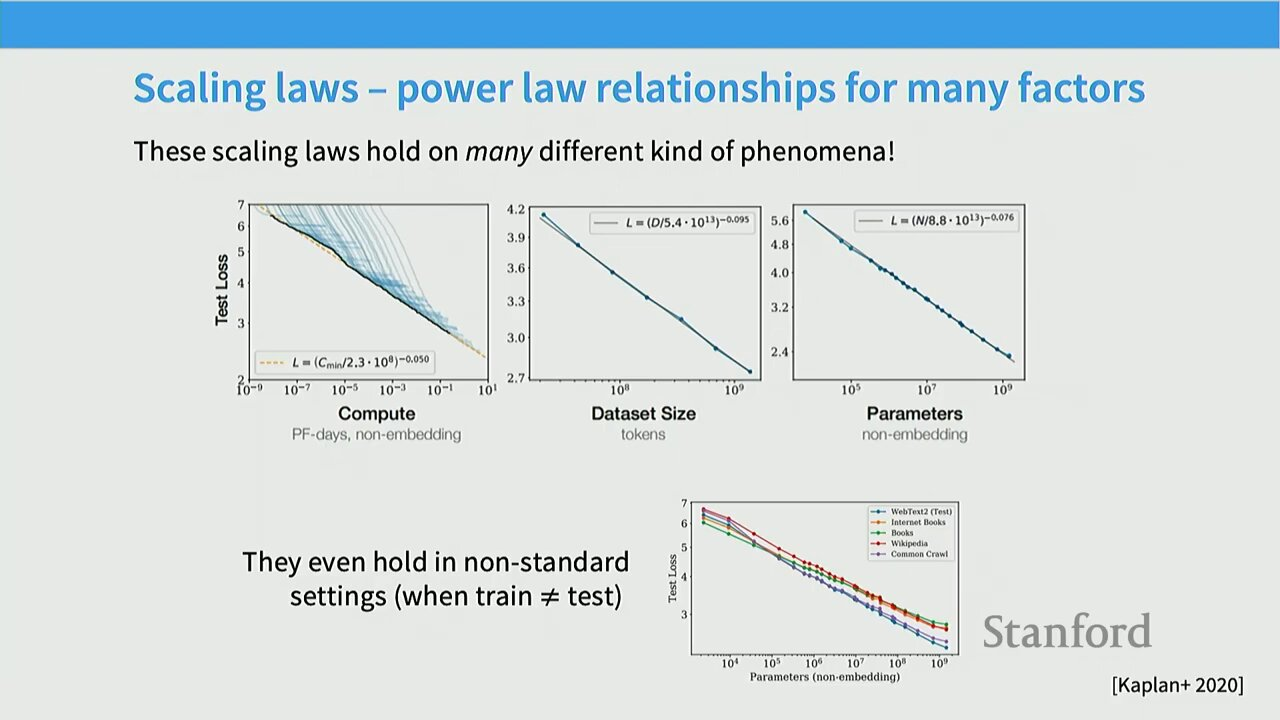
\includegraphics[width=0.92\textwidth]{figures/fig_kaplan_scaling_vars.jpg}
\caption{Kaplan et al.\ 2020《Scaling Laws for Neural Language Models》：在 compute $C$、数据 $D$、参数 $N$ 三个变量上 loss 都呈幂律。\protect\footnotemark}
\end{figure}
\footnotetext{视频画面时间区间：00:12:30--00:13:00。}

Kaplan 论文的贡献是把上述规律\textbf{系统化}到 LLM 时代：固定其他变量足够大（远离饱和）时，loss 关于单个变量都呈幂律。

\begin{practicebox}{Kaplan 单变量缩放的实验设计要点}
单变量缩放成立的前提是\textbf{另一变量保持"远离饱和"足够远}。例如，研究 loss vs $N$ 时，必须让 $D$ 远超该 $N$ 的饱和点，否则测量到的衰减是被数据瓶颈拉平后的"假斜率"。这是后续做 scaling law 实验的\textbf{最重要设计纪律}。
\end{practicebox}

\section{理论起点：为什么是幂律？}

Percy 接下来追问一个根本问题：\textbf{为什么是幂律、而不是指数或对数}？他给出两个具有启发性的理论模型——均值估计与非参数回归。

\subsection{均值估计：最简单的 scaling law 例子}

\begin{figure}[H]
\centering
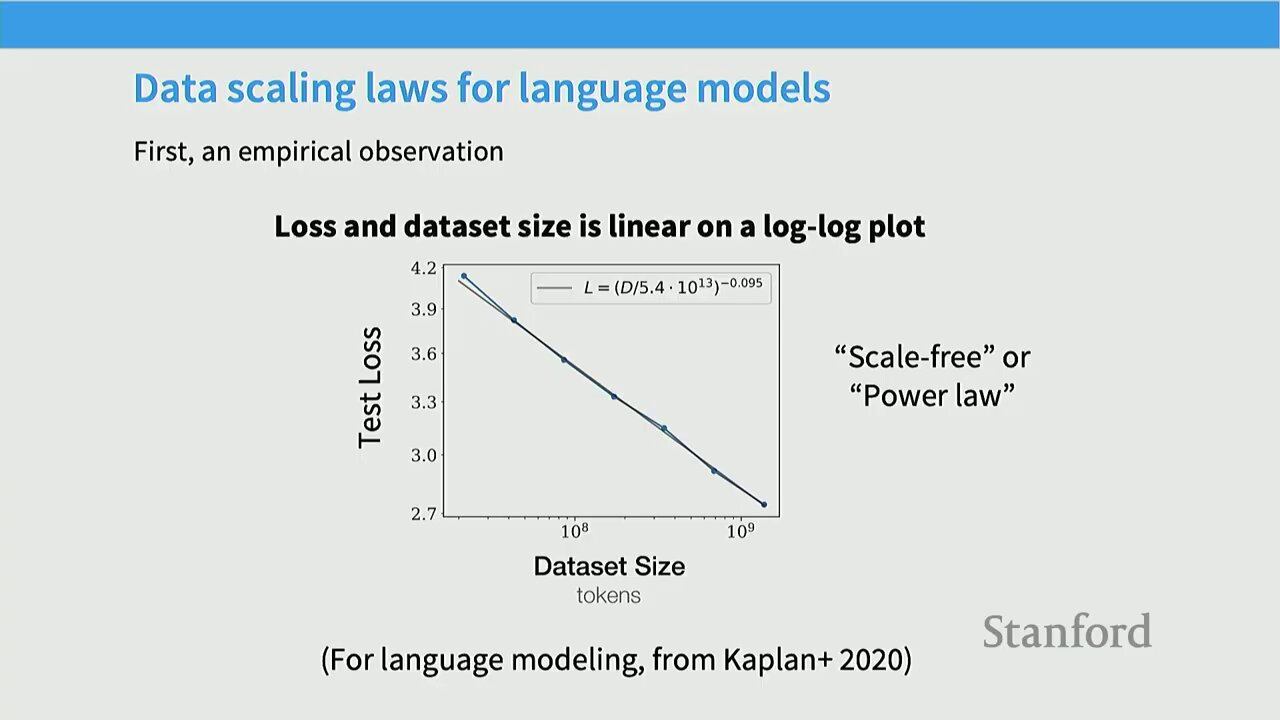
\includegraphics[width=0.88\textwidth]{figures/fig_mean_estimation_powerlaw.jpg}
\caption{均值估计是最简洁的 scaling law 例子：从高斯分布采 $n$ 个样本估均值，估计误差方差 $\sigma^2/n$，log-log 下斜率 $-1$。\protect\footnotemark}
\end{figure}
\footnotetext{视频画面时间区间：00:14:45--00:15:15。}

考虑最简单的估计问题：从 $\mathcal{N}(\mu,\sigma^2)$ 中独立采样 $n$ 个点 $x_1,\ldots,x_n$，用样本均值 $\bar{x}=\frac{1}{n}\sum x_i$ 估 $\mu$。估计误差的方差为
\[
\mathrm{Var}(\bar{x}) \;=\; \frac{\sigma^2}{n}.
\]
取 log：
\[
\log \mathrm{Var}(\bar{x}) \;=\; \log \sigma^2 \;-\; \log n,
\]
即 log-log 下斜率 $-1$。\textbf{幂律在这里是中心极限定理的直接推论}，并不是奇特的统计现象。

\subsection{实测指数与理论的偏离}

\begin{figure}[H]
\centering
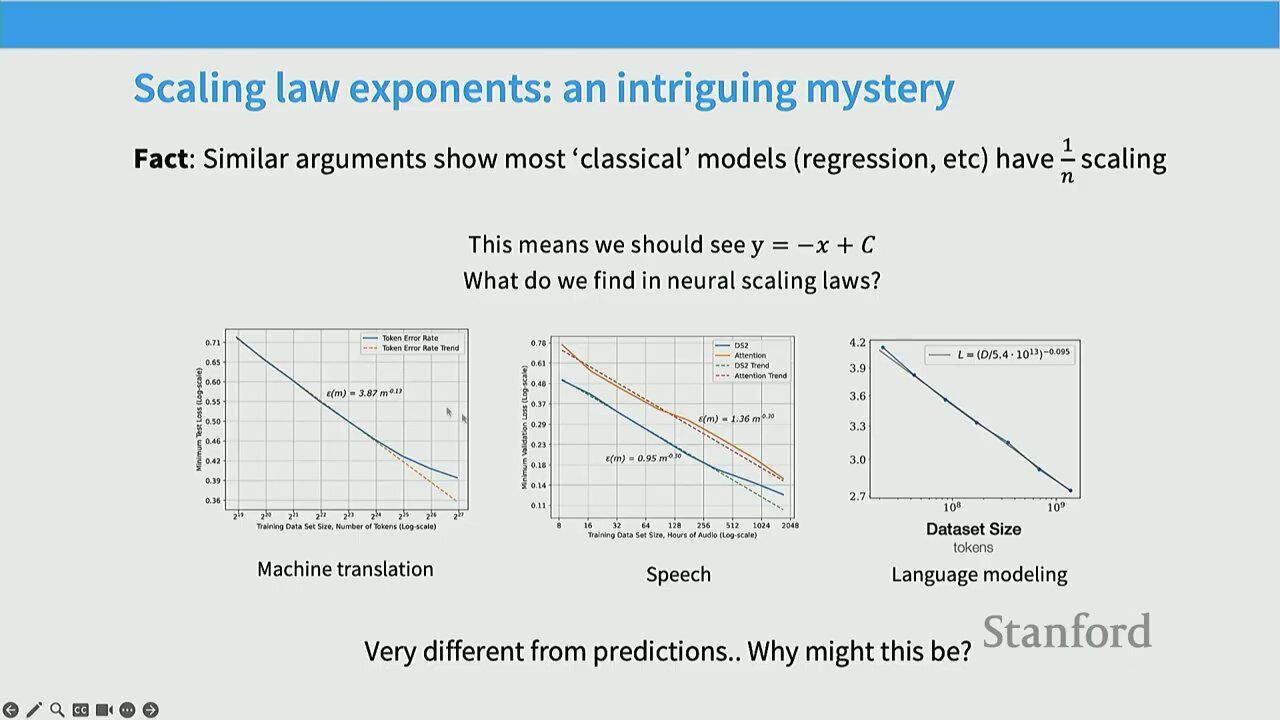
\includegraphics[width=0.88\textwidth]{figures/fig_empirical_exponents.jpg}
\caption{不同任务的实测 scaling 指数：MT $\approx 0.13$、speech $\approx 0.3$、LM $\approx 0.95$，都比理论的 $-1$（均值估计）或 $-0.5$（PAC 界）慢得多。\protect\footnotemark}
\end{figure}
\footnotetext{视频画面时间区间：00:17:15--00:17:45。}

\begin{importantbox}{理论与实测的鸿沟}
理论界 $O(1/\sqrt{n})$（$p=0.5$）在真实任务上几乎从不出现；实测 $p$ 普遍在 $0.05$ 到 $1$ 之间，跨度极大。这告诉我们：\textbf{真实的 scaling 指数强烈依赖任务的"内在难度"，没有放之四海皆准的理论值}。
\end{importantbox}

\subsection{非参数回归与内在维度}

\begin{figure}[H]
\centering
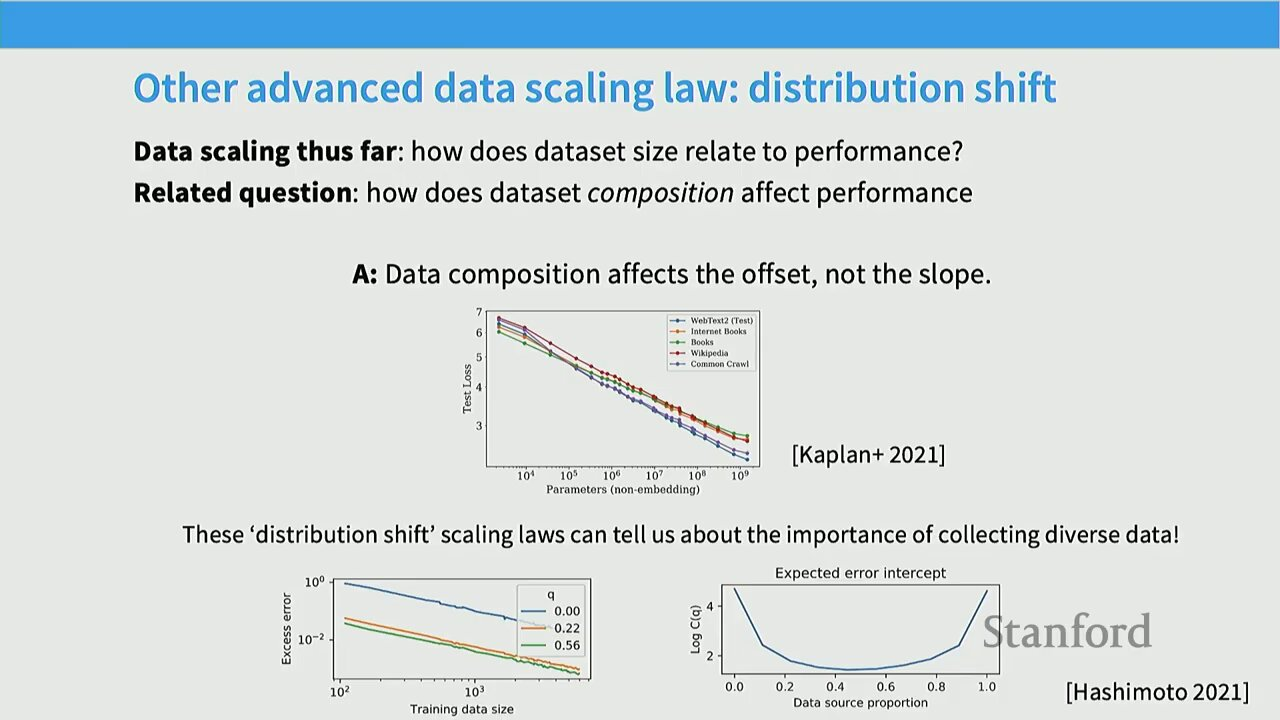
\includegraphics[width=0.88\textwidth]{figures/fig_intrinsic_dimension.jpg}
\caption{非参数回归（box-counting）论证：$d$ 维空间下估计误差 $\sim n^{-1/(d+1)}$。指数直接反映数据的\emph{内在维度}。\protect\footnotemark}
\end{figure}
\footnotetext{视频画面时间区间：00:21:15--00:21:45。}

为解释为什么实测 $p$ 这么小，Percy 引入非参数回归论证：若数据流形真实维度为 $d$，则局部估计的误差率满足
\[
\text{MSE} \;\sim\; n^{-2/(d+1)}.
\]
当 $d$ 很大时（比如 LM 中真实数据分布的高维度），指数 $2/(d+1)$ 会非常小，正好对应实测到的缓慢衰减。

\begin{knowledgebox}{内在维度（intrinsic dimensionality）的解读}
这给出了一个直观故事：\textbf{衰减指数越小 $\Leftrightarrow$ 任务内在维度越高 $\Leftrightarrow$ 学起来越难}。LM 的 $p\approx 0.95$ 之所以"相对大"，是因为 next-token prediction 在每一步都是相对受限的局部估计；而 MT 的 $p\approx 0.13$ 之小，是因为翻译需要同时建模语法、语义、对齐——内在维度高得多。
\end{knowledgebox}

\section{模型规模缩放：架构与优化器}

把目光从数据转到模型，Percy 展示了一系列关于\textbf{架构与优化器选择是否改变 scaling 曲线}的实证。

\subsection{架构选择：LSTM vs Transformer}

\begin{figure}[H]
\centering
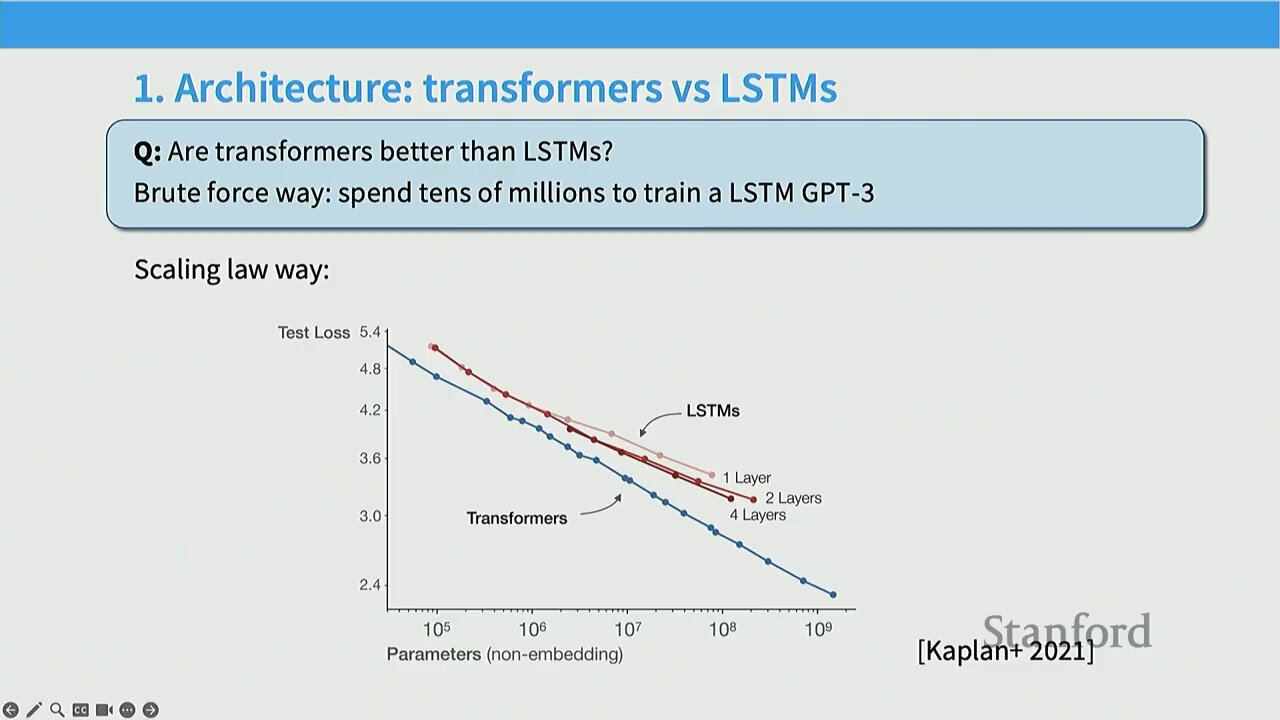
\includegraphics[width=0.92\textwidth]{figures/fig_lstm_vs_transformer.jpg}
\caption{Hestness 的跨架构 scaling 对比：LSTM 与 Transformer 在 log-log 下的斜率几乎一致，差异主要体现在常数倍数（LSTM 有约 $15\times$ 的 compute 惩罚）。\protect\footnotemark}
\end{figure}
\footnotetext{视频画面时间区间：00:27:15--00:27:45。}

\begin{importantbox}{架构主要改变常数、而非指数}
跨多个 compute 阈值的对比显示：不同架构的 scaling 曲线常常\textbf{斜率相近、只差常数倍数}。LSTM 相比 Transformer 大约有 $15\times$ 的 compute 惩罚，但幂律形状一致。\textbf{这意味着架构选择决定"效率"，scaling law 决定"轨迹"}。
\end{importantbox}

这一发现对工程意义重大：\textbf{可以放心用小规模实验比较架构的常数效率}，然后假设该效率差在大规模下保持。

\subsection{优化器：SGD vs Adam}

\begin{figure}[H]
\centering
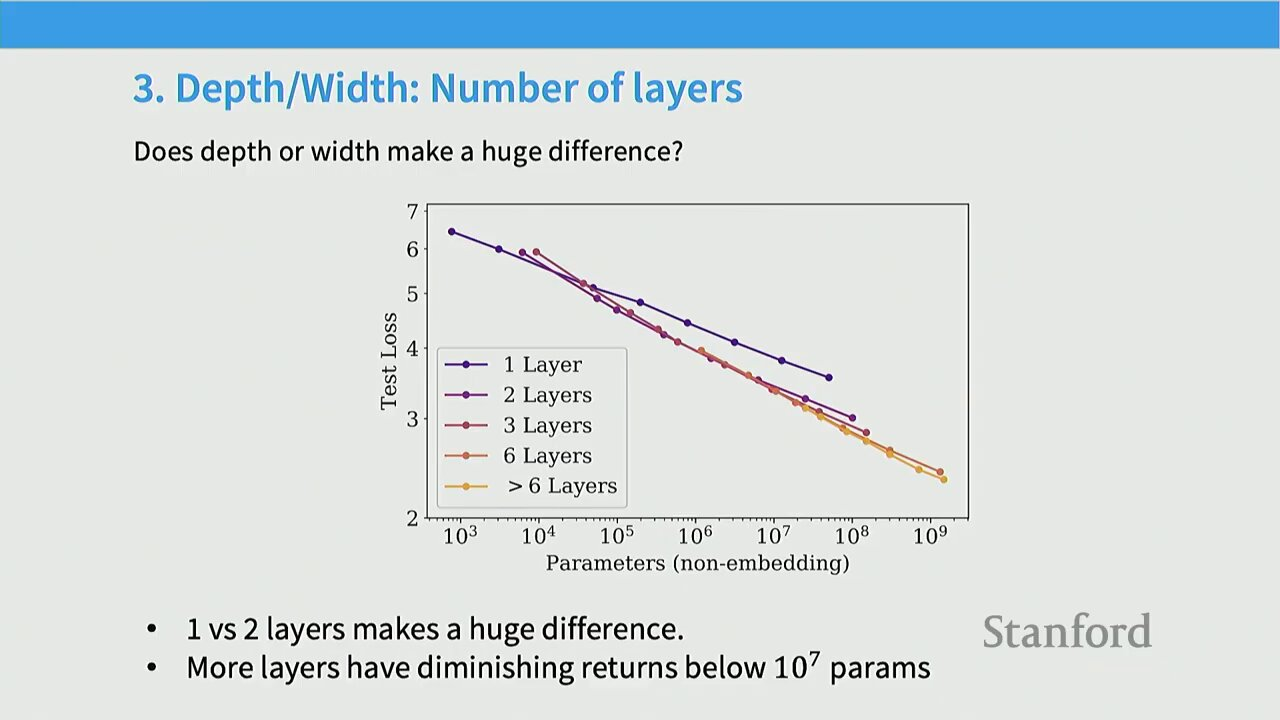
\includegraphics[width=0.88\textwidth]{figures/fig_optimizer_sgd_adam.jpg}
\caption{优化器 scaling 对比：SGD 与 Adam 在不同 dataset size 下呈常数效率差，Adam 在 LM 任务上更优。\protect\footnotemark}
\end{figure}
\footnotetext{视频画面时间区间：00:29:45--00:30:15。}

优化器选择也呈现类似的"常数偏移"特征：\textbf{Adam 在大多数 LM 任务上稳定优于 SGD 一个常数因子}，但同样不改幂律指数。

\subsection{深度-宽度比（Aspect Ratio）}

\begin{figure}[H]
\centering
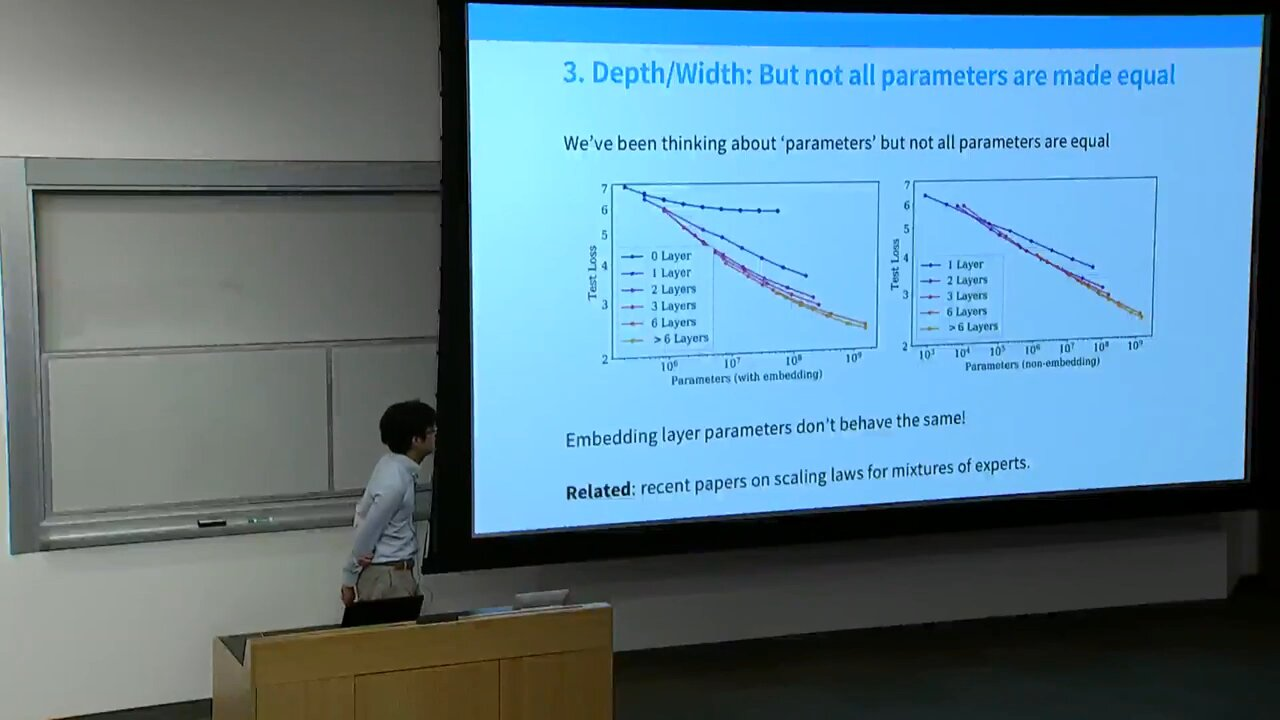
\includegraphics[width=0.92\textwidth]{figures/fig_aspect_ratio.jpg}
\caption{Kaplan 的 aspect ratio 分析：在 50M / 270M / 1.5B 三个规模上扫描深度-宽度比，发现曲线形状相似、最优值都落在 10--100 之间。\protect\footnotemark}
\end{figure}
\footnotetext{视频画面时间区间：00:30:45--00:31:15。}

Kaplan 对模型形状做了细致切片：在多个 compute 阈值下扫描"宽盆"（width）vs"深盆"（depth），发现最优 aspect ratio 在 10 到 100 之间，且\textbf{跨规模保持稳定}。这给出一个重要工程结论：

\begin{practicebox}{超参可迁移性（hyperparameter transfer）}
既然曲线形状相似，就可以\textbf{在小模型上确定 aspect ratio、head dim、FFN ratio 等结构超参，再直接迁移到大模型}。这把"选大模型形状"的成本从 trillion 级实验降到了 million 级。
\end{practicebox}

\subsection{Non-embedding 参数：被忽视的细节}

\begin{figure}[H]
\centering
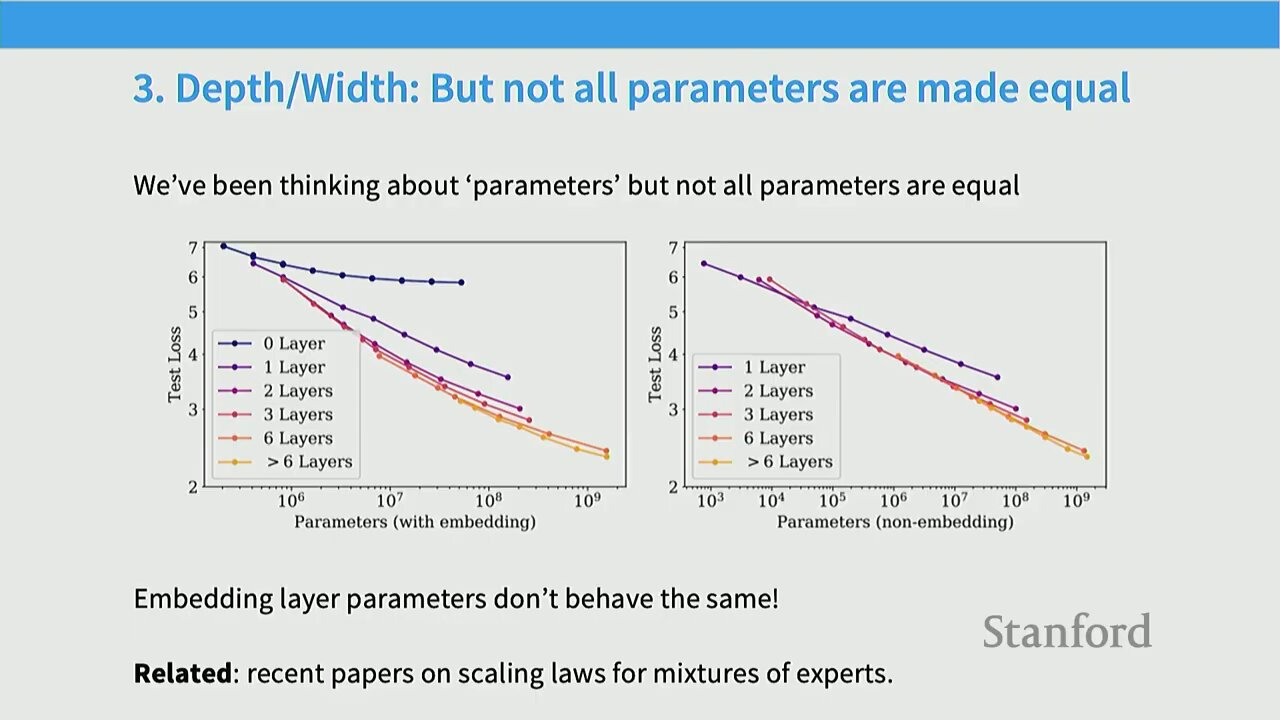
\includegraphics[width=0.88\textwidth]{figures/fig_non_embedding_params.jpg}
\caption{关键细节：embedding 参数与 non-embedding 参数行为不同。Kaplan 发现只用 non-embedding 参数 $N$ 才能得到干净的幂律。\protect\footnotemark}
\end{figure}
\footnotetext{视频画面时间区间：00:31:45--00:32:15。}

Kaplan 的一个看似细微但影响重大的发现是：\textbf{embedding 参数与 transformer body 的 non-embedding 参数在 scaling 行为上是不同的}。把 embedding 也算进 $N$ 会让幂律变"脏"，因此他们规定：

\[
N \;=\; \text{non-embedding 参数总量}.
\]

后续文献基本沿用这一定义。

\begin{knowledgebox}{MoE 中的"参数"概念同样模糊}
Percy 在课上提到，最近 MoE（Mixture of Experts）的论文也在重演类似问题：稀疏激活的参数"算几份"？这些工作都试图推导\textbf{等效 dense 参数量}来归一化比较，思路与 Kaplan 的"只数 non-embedding"一脉相承。
\end{knowledgebox}

\subsection{超参切片（Hyperparameter Slices）}

\begin{figure}[H]
\centering
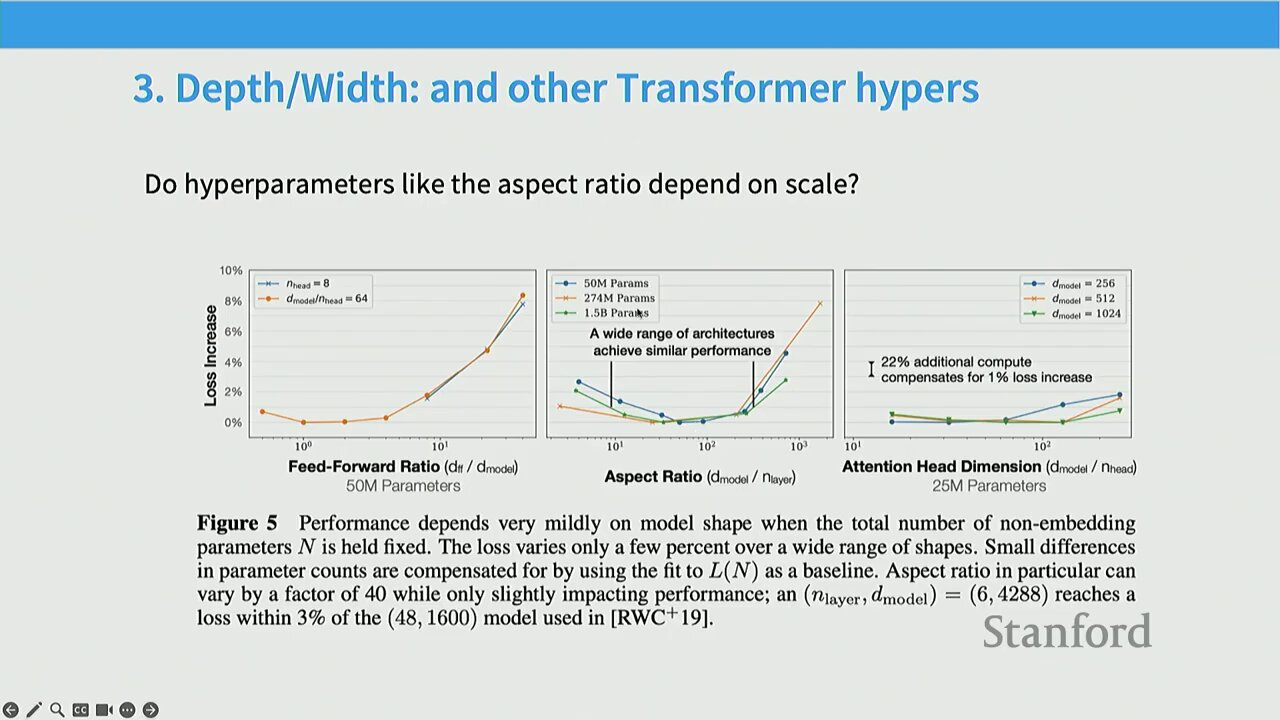
\includegraphics[width=0.92\textwidth]{figures/fig_hyperparam_slices.jpg}
\caption{Scale-aware 超参选择：在多个 compute 切片下扫描 FFN dim ratio / attention head dim，最优值在不同 compute 下保持相似——这正是 hyperparameter transfer 成立的实证基础。\protect\footnotemark}
\end{figure}
\footnotetext{视频画面时间区间：00:33:15--00:33:45。}

Percy 强调，Kaplan 论文最值得反复看的就是这些切片图（尤其是 aspect ratio 那张）：他们不是简单"放大模型"，而是\textbf{在 50M / 270M / 1.5B 三个规模上分别扫描超参，验证最优值跨规模保持稳定}。

\section{Batch Size 与学习率：两个特殊超参}

并非所有超参都能"切片迁移"。Percy 指出，\textbf{batch size 和 learning rate 是两个例外}，它们的 scale 行为需要单独处理。

\subsection{Batch size 与 noise scale}

\begin{figure}[H]
\centering
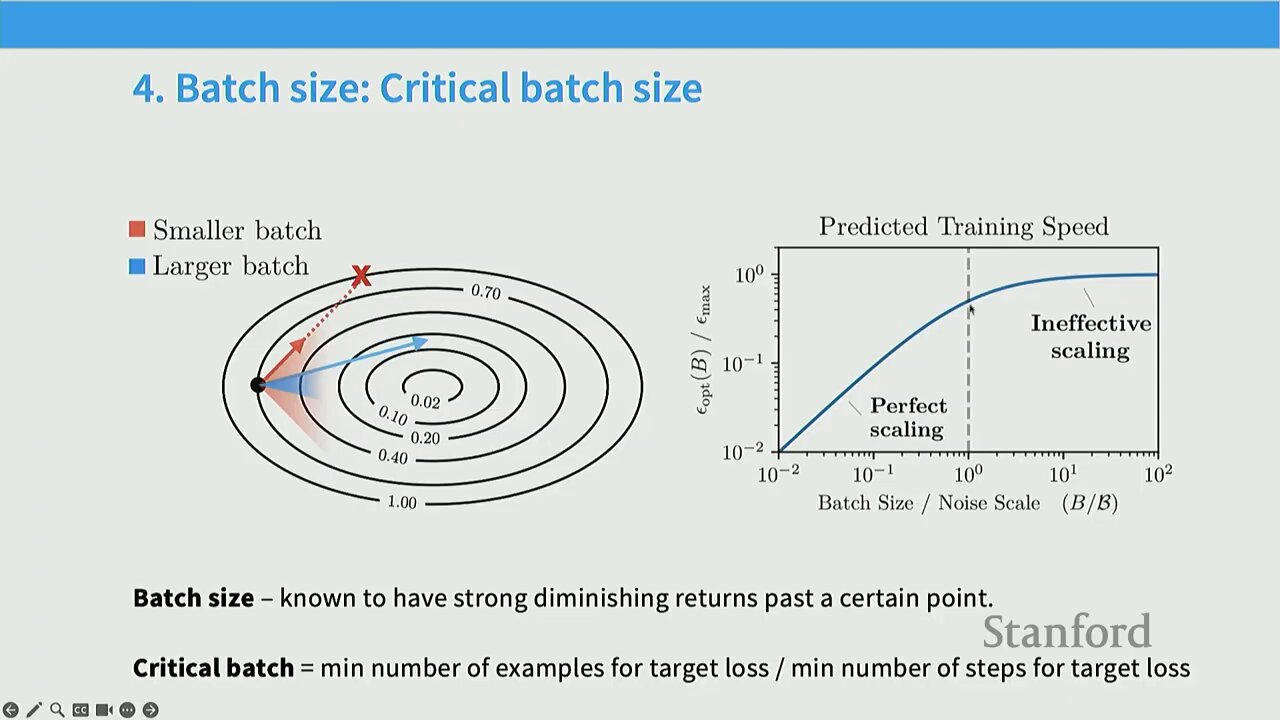
\includegraphics[width=0.88\textwidth]{figures/fig_batch_noise_scale.jpg}
\caption{Batch size 与 gradient noise scale：当 batch 小于 noise scale 时，增 batch 等价于多走梯度步；超过后边际递减。\protect\footnotemark}
\end{figure}
\footnotetext{视频画面时间区间：00:35:15--00:35:45。}

为什么 batch size 特殊？因为它直接控制\textbf{梯度估计的方差}。当 batch size $B$ 小于某个临界 noise scale $B_{\text{noise}}$ 时：
\[
\text{增 batch} \;\approx\; \text{多走有效梯度步},
\]
即计算效率高；超过 $B_{\text{noise}}$ 后，再多 batch 只是在重复相同梯度信息，边际收益骤降。

\subsection{Critical batch size}

\begin{figure}[H]
\centering
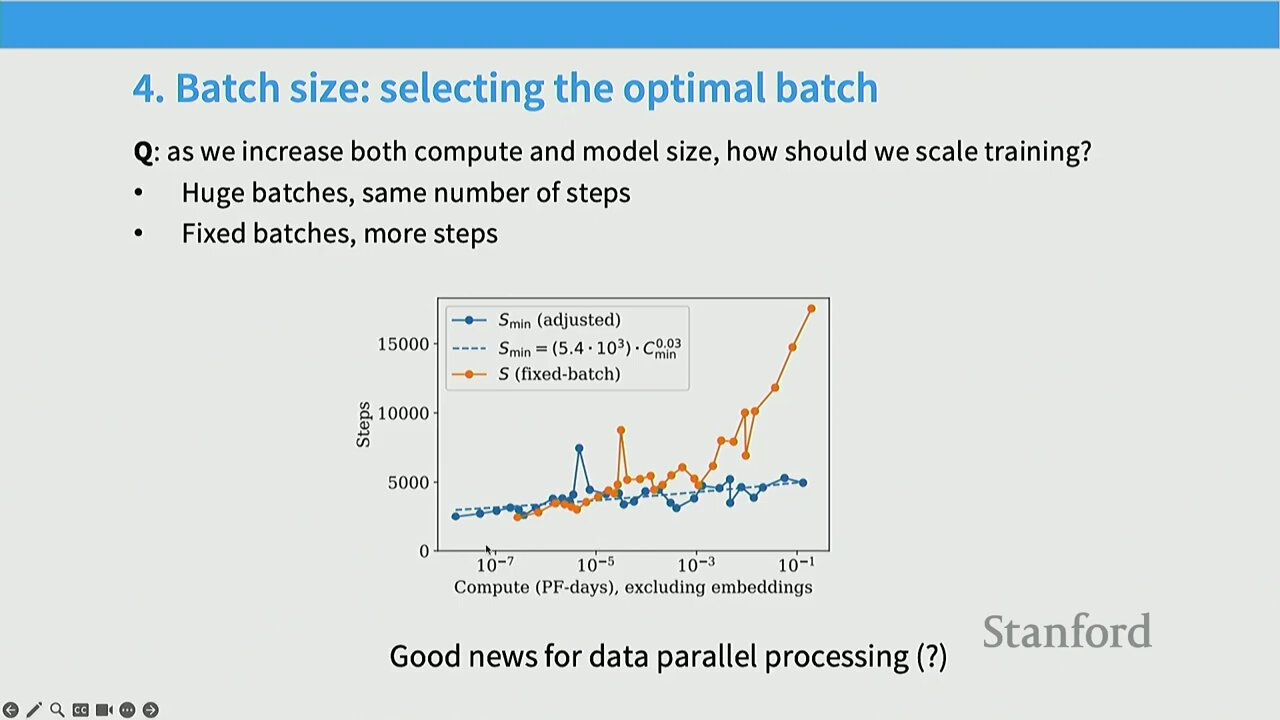
\includegraphics[width=0.88\textwidth]{figures/fig_critical_batch_size.jpg}
\caption{Critical batch size：loss target 越小（即追求越好），critical batch size 越大；Llama 3 训练中会在训练过程动态增大 batch。\protect\footnotemark}
\end{figure}
\footnotetext{视频画面时间区间：00:37:15--00:37:45。}

\begin{importantbox}{Critical batch size 与训练策略}
Critical batch size 不是常数，而是\textbf{loss target 的函数}：loss target 越低（模型越好），$B^{\*}$ 越大。这就解释了 Llama 3 训练后期会主动\textbf{动态增大 batch size}——在更后期、loss 更低的阶段，更大的 batch 才仍是"有效"的。
\end{importantbox}

\subsection{学习率 scaling}

\begin{figure}[H]
\centering
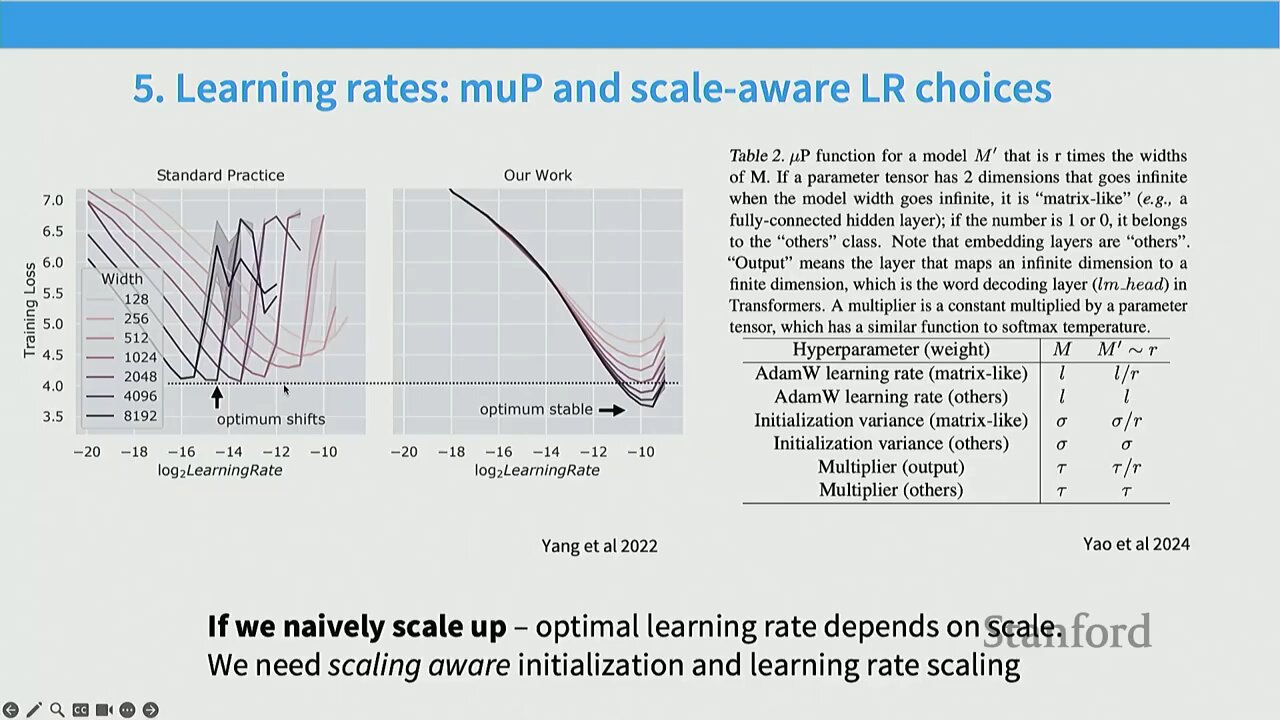
\includegraphics[width=0.88\textwidth]{figures/fig_learning_rate_scaling.jpg}
\caption{学习率 scaling：标准 parameterization 下最优 LR 随宽度衰减（约 $\propto 1/\text{width}$），可用 scaling law 拟合最优 LR 曲线。\protect\footnotemark}
\end{figure}
\footnotetext{视频画面时间区间：00:39:15--00:39:45。}

学习率同样不能简单"小模型上选好就迁移"。在标准 parameterization 下，最优学习率\textbf{随宽度衰减}（近似 $\propto 1/\text{width}$）。可以用 scaling law 拟合这条最优 LR 曲线，再外推到大模型。

\begin{knowledgebox}{muP（Maximal Update Parameterization）}
一种更激进的解法是 Yang 提出的 \textbf{muP}：通过精心协调初始化方差与学习率的缩放规则，让\textbf{最优超参在任意宽度下都保持不变}。这样小模型上选好的 LR 可以零代价迁移到大模型。muP 已是当代大模型训练的标准工具之一。
\end{knowledgebox}

\section{Perplexity 与下游任务：scaling 的边界}

\begin{figure}[H]
\centering
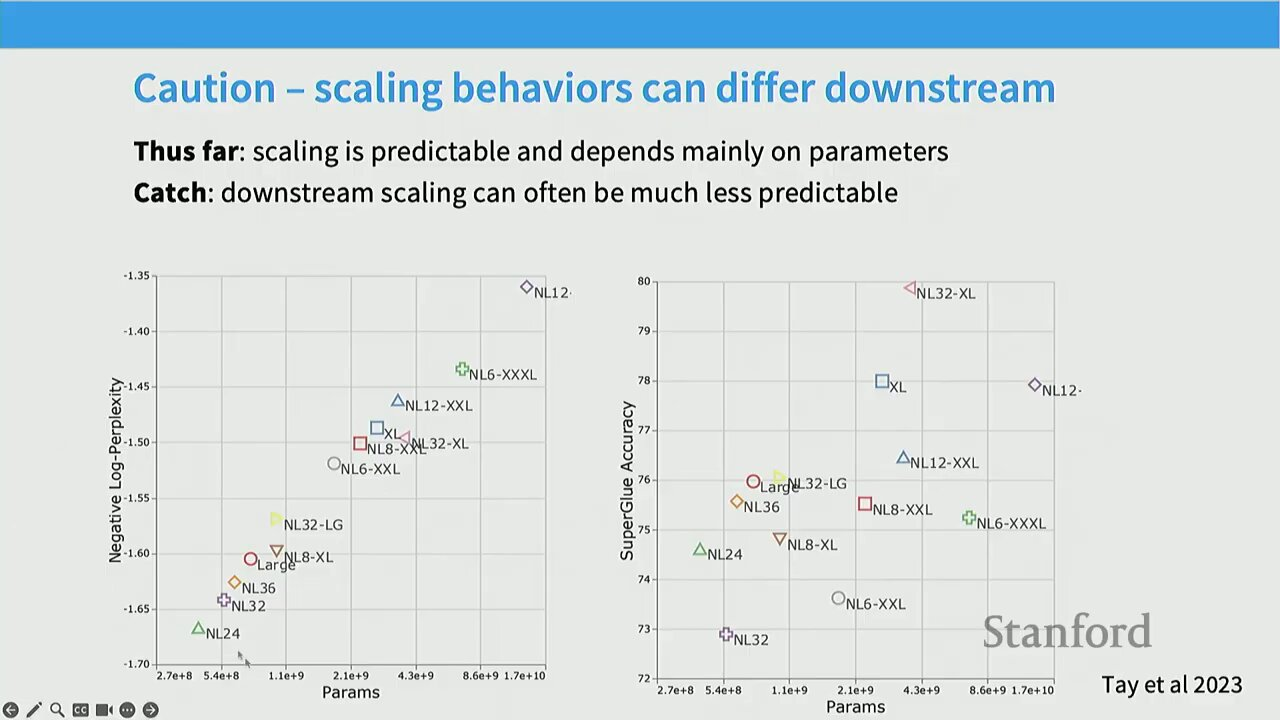
\includegraphics[width=0.92\textwidth]{figures/fig_downstream_vs_perplexity.jpg}
\caption{重要警告：perplexity 的 scaling 极干净（几乎只取决于总 compute），但下游任务（如 SuperGLUE）的 scaling 远不可预测，且不同架构差异明显。\protect\footnotemark}
\end{figure}
\footnotetext{视频画面时间区间：00:43:45--00:44:15。}

\begin{warningbox}{不要把 perplexity scaling 直接外推到下游任务}
Perplexity（next-token cross-entropy）是 scaling law 文献的"默认指标"，因为它单调、平滑、跨架构稳定。但 Percy 在此郑重警告：\textbf{真实关心的下游能力（推理、问答、SuperGLUE 等）的 scaling 远没有 perplexity 那么干净}。不同架构在 perplexity 上接近，在下游任务上可能差异显著。
\end{warningbox}

实践含义：scaling law 给的是\textbf{训练 loss 的轨迹}，而"loss 更低 $\Rightarrow$ 下游更好"的桥梁需要单独验证。这是当代 scaling law 研究的开放问题之一。

\section{联合缩放：从单变量到 (N, D) 曲面}

前面分别讨论了 loss 关于 $N$、$D$、$C$ 的单变量幂律。但真正的工程问题是：\textbf{在固定 compute 预算下，如何联合优化 $N$ 和 $D$}？这需要联合 scaling 曲面。

\subsection{Rosenfeld 的联合曲面拟合}

\begin{figure}[H]
\centering
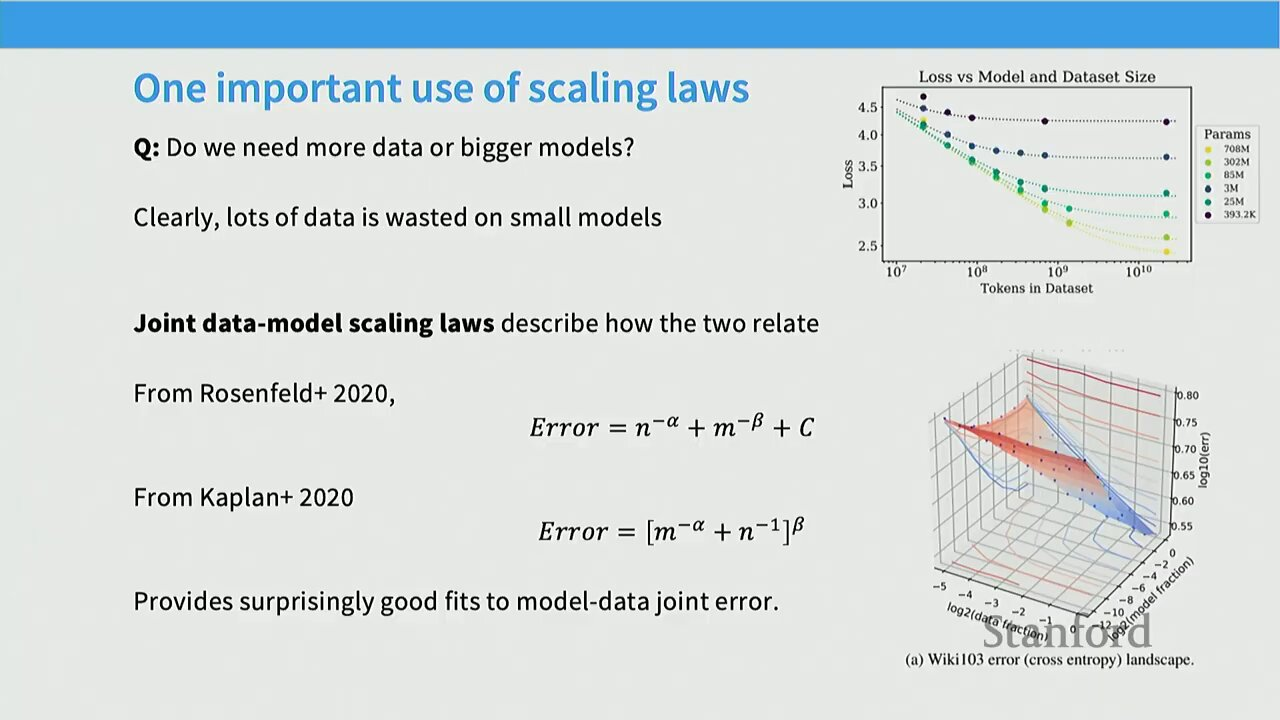
\includegraphics[width=0.92\textwidth]{figures/fig_rosenfeld_joint.jpg}
\caption{Rosenfeld 的 3D 联合曲面：$x$ 轴数据量、$y$ 轴模型大小、$z$ 轴 loss。拟合曲面几乎完美贴合所有数据点，且从小规模外推大规模误差极小。\protect\footnotemark}
\end{figure}
\footnotetext{视频画面时间区间：00:47:45--00:48:15。}

Rosenfeld 等人提出一个简洁的两项相加形式来拟合联合 loss：

\[
L(N,D) \;=\; \alpha \;+\; \frac{\beta}{N^{p}} \;+\; \frac{\gamma}{D^{q}}.
\]

其中 $\alpha$ 仍是不可约误差，两项分别表示\textbf{参数不足}和\textbf{数据不足}造成的可约误差。

\begin{importantbox}{为何这个 ad-hoc 形式如此有效}
Percy 坦言这个函数形式\textbf{没有严格的"自顶向下"理论依据}——它是从 hat 里掏出来的。但实测中它对 (N, D) 联合 loss 的拟合精度惊人：用小规模点拟合后外推到大 (N, D)，预测值与实测值在 ImageNet、WikiText 上都几乎贴线。这正是 scaling law 作为\textbf{经验工程工具}而非理论的魅力。
\end{importantbox}

\subsection{Kaplan 的联合 compute-data 视角}

\begin{figure}[H]
\centering
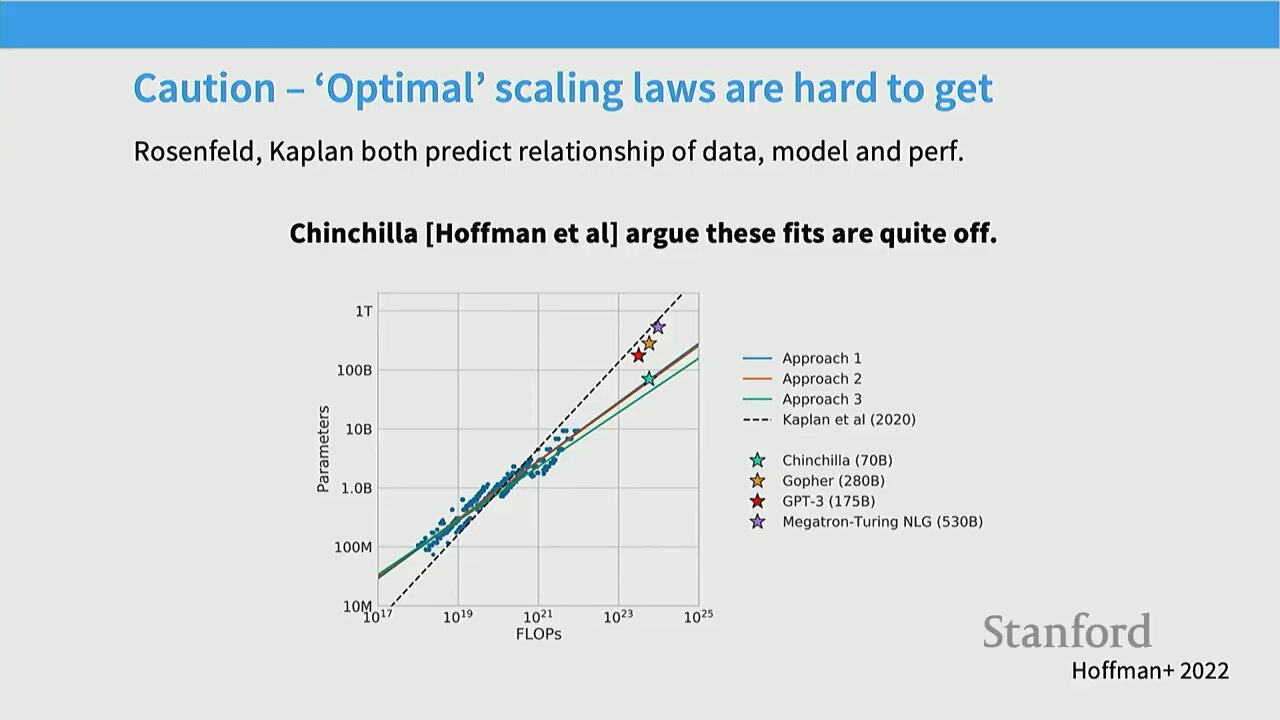
\includegraphics[width=0.92\textwidth]{figures/fig_kaplan_joint_compute.jpg}
\caption{Kaplan 的联合 compute-data scaling：参数为 $x$ 轴、颜色代表不同 compute 预算，数据维度被隐式调整以匹配总 compute。\protect\footnotemark}
\end{figure}
\footnotetext{视频画面时间区间：00:50:45--00:51:15。}

Kaplan 的版本以参数量为 $x$ 轴、不同 compute 预算用不同颜色表示：\textbf{沿一条颜色曲线移动}意味着固定 compute、改变 $N$（同时数据 $D$ 被隐式调整以守恒总 compute）。这给出了"给定预算下最优 $N$"的可视化基础——为下一节的 Chinchilla 分析铺路。

\section{为什么 Kaplan 低估了数据需求（cosine LR 问题）}

\begin{figure}[H]
\centering
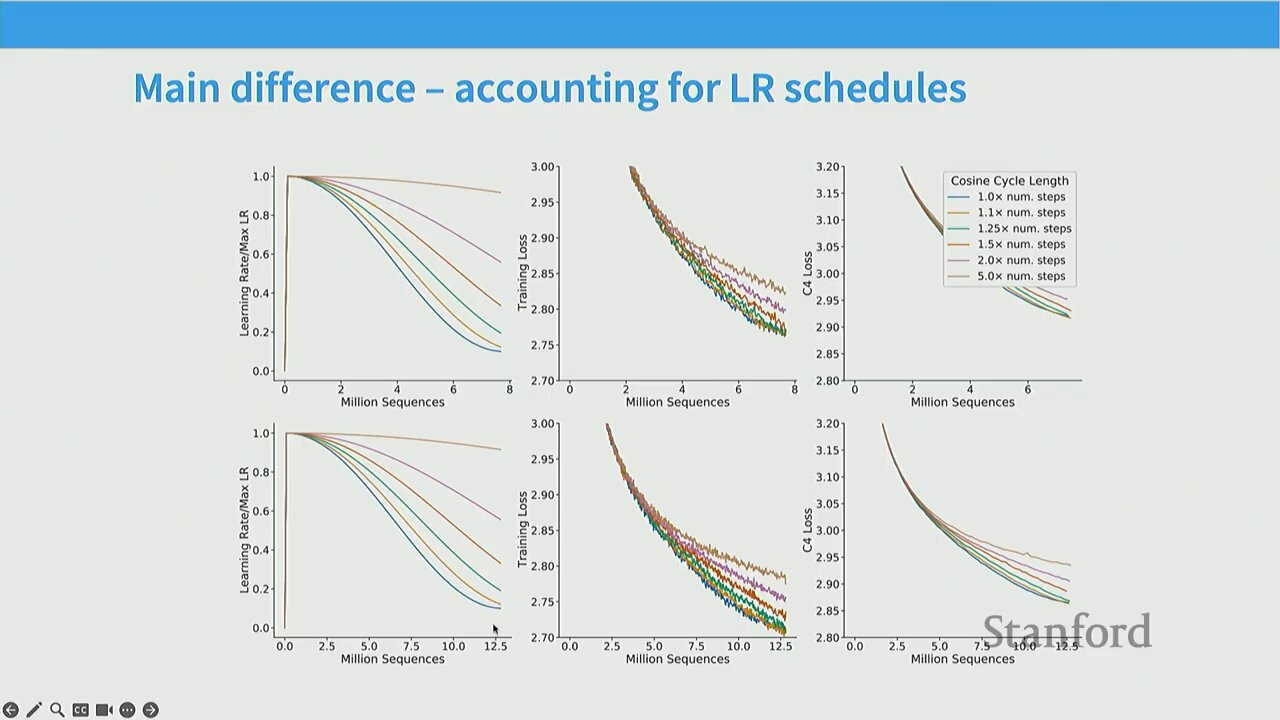
\includegraphics[width=0.88\textwidth]{figures/fig_cosine_lr_issue.jpg}
\caption{Kaplan 低估数据需求的关键原因之一：cosine LR schedule 不能截断。把一个长 schedule 截到中段，不等于从头训到中段。\protect\footnotemark}
\end{figure}
\footnotetext{视频画面时间区间：00:52:45--00:53:15。}

Kaplan 论文得出"参数应增长快于数据"的结论，意味着 Chinchilla 之前业界普遍\textbf{训练得参数过多、数据过少}（GPT-3 就是最典型的代表，约 2 tokens/parameter）。Percy 在此揭示 Kaplan 偏差的关键技术原因：

\begin{warningbox}{Cosine LR schedule 的截断问题}
Kaplan 在做 scaling law 实验时，用了一种"训练到不同步数再读 loss"的做法。但 cosine LR schedule 是\textbf{与总训练步数强绑定的}：把一个 100k 步的 cosine schedule 在 50k 步处截断读 loss，得到的是"learning rate 还在中段、远未退火到 0"的模型，\textbf{并不等于}一个从一开始就计划只训 50k 步、schedule 已完整退火的模型。

这个偏差让 Kaplan 系统性地\textbf{高估了"用更多参数训练更少步"的效率}，从而得出"参数应增长快于数据"的偏倚结论。
\end{warningbox}

Chinchilla 论文修正了这一点（以及其他方法论问题），得出了几乎相反的结论。

\section{Chinchilla：三种方法、一个结论}

Chinchilla（Hoffmann et al.\ 2022）是 scaling law 文献的里程碑。Percy 用三种独立方法分别重建了 compute-optimal 点，并强调\textbf{三种方法殊途同归}这一事实本身就是结论稳健性的最强证据。

\subsection{Method 1：Minimum Envelope}

\begin{figure}[H]
\centering
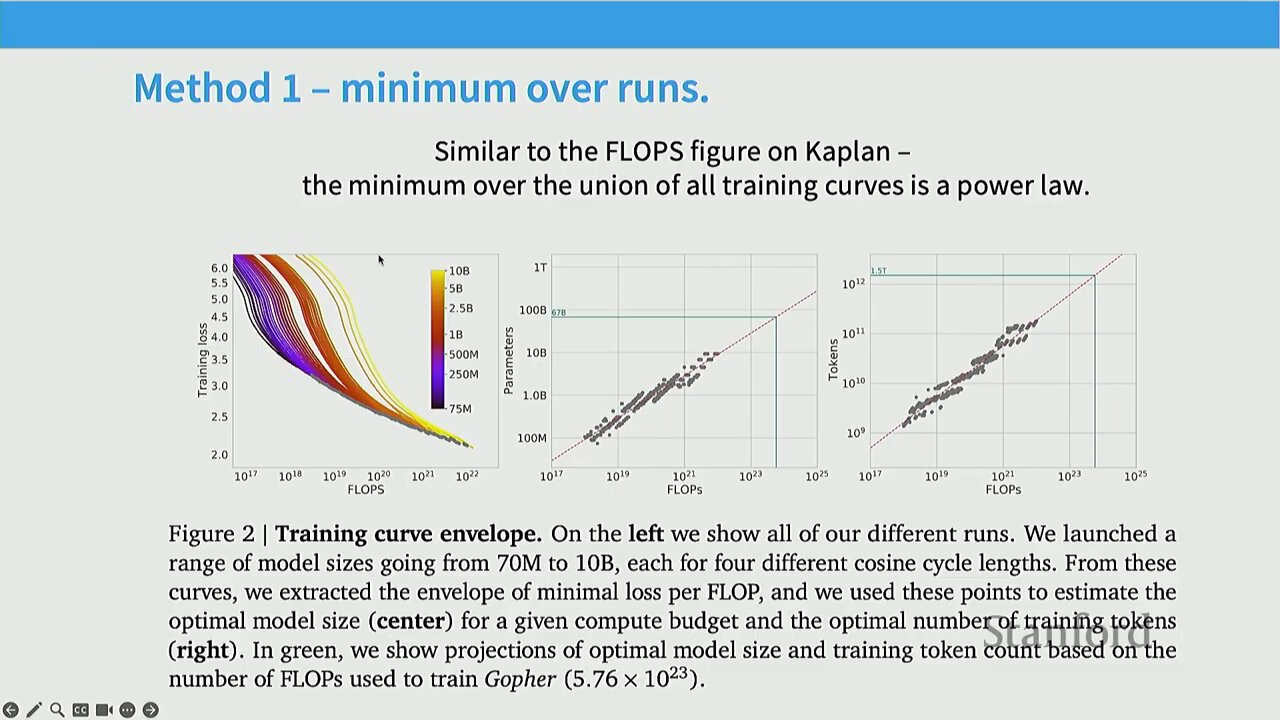
\includegraphics[width=0.92\textwidth]{figures/fig_chinchilla_method1.jpg}
\caption{Chinchilla Method 1：取所有训练曲线的下包络（minimum envelope），提取每个 compute 预算下的最优 (N, D) 组合。\protect\footnotemark}
\end{figure}
\footnotetext{视频画面时间区间：00:54:45--00:55:15。}

Method 1 的思路最直接：\textbf{对每个 compute 预算 $C$，找出在所有 (N, D) 组合里 loss 最低的那个点}，再把这些最优点的 $N^{\*}(C)$ 与 $D^{\*}(C)$ 拟合为 $C$ 的幂律：
\[
N^{\*}(C) \;\propto\; C^{a}, \quad D^{\*}(C) \;\propto\; C^{b}.
\]
Chinchilla 测得 $a \approx b \approx 0.5$，即\textbf{参数和数据应等比例增长}。

\subsection{Method 2：IsoFLOP 曲线}

\begin{figure}[H]
\centering
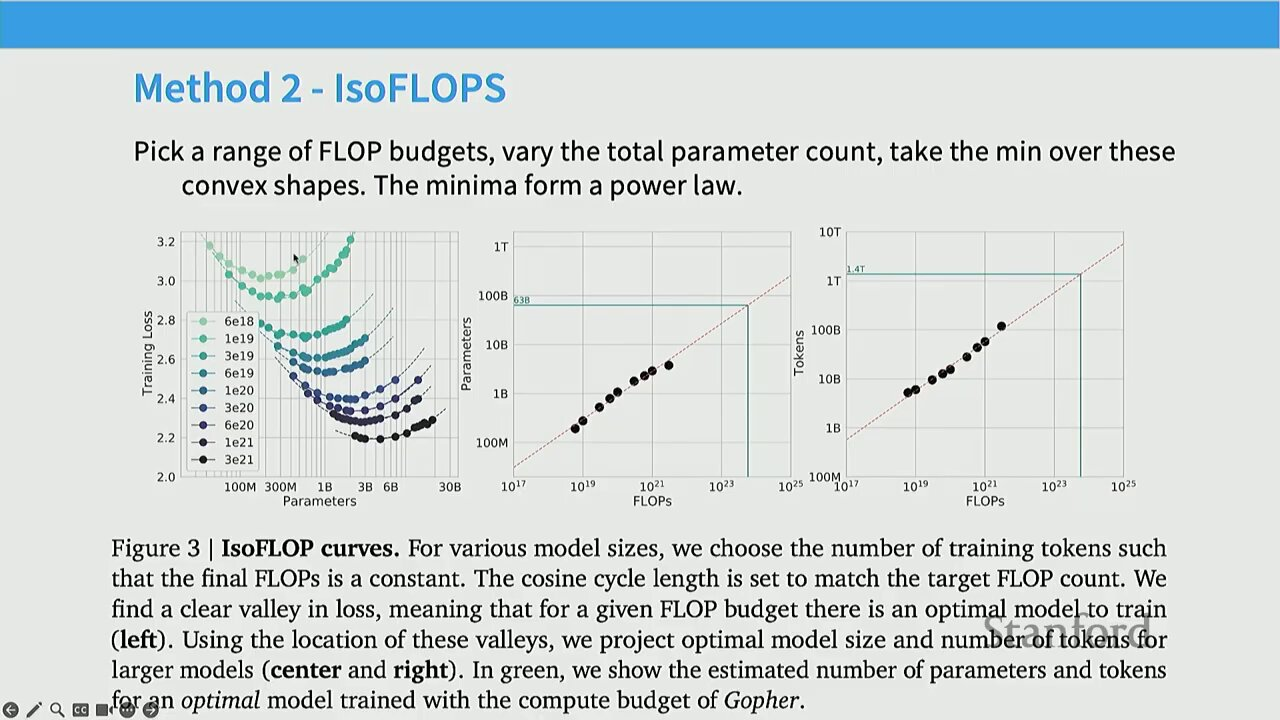
\includegraphics[width=0.92\textwidth]{figures/fig_chinchilla_isoflop.jpg}
\caption{Chinchilla Method 2（IsoFLOP 曲线）：固定每个 compute 水平扫模型大小，取每条曲线最低点。最优模型约 63--67B。\protect\footnotemark}
\end{figure}
\footnotetext{视频画面时间区间：00:56:45--00:57:15。}

Method 2 把每个固定 FLOPs 水平单独画一条 loss-vs-$N$ 曲线（IsoFLOP contour），然后\textbf{取每条曲线的最低点}（或用二次拟合求最小值）。对 Chinchilla 的目标 FLOPs（约 $10^{21}$），三种方法都给出 $N^{\*}\approx 63$--$67\,\text{B}$。

\begin{practicebox}{IsoFLOP 分析的实操步骤}
\begin{enumerate}
\item 选定一组 compute 预算 $\{C_1, C_2, \ldots\}$；
\item 对每个 $C_i$，训练一族不同 $N$ 的模型（每个都恰好消耗 $C_i$ FLOPs）；
\item 画 loss vs $N$，取最低点 $(N^{\*}_i, L^{\*}_i)$；
\item 把 $\{(N^{\*}_i, C_i)\}$ 拟合为幂律，得 $N^{\*}(C)$。
\end{enumerate}
Percy 特别指出：\textbf{IsoFLOP 曲线的干净程度"令人惊讶"}——即便今天看，依然非常美观、可复现性极高。
\end{practicebox}

\subsection{Method 3：参数化曲线拟合}

\begin{figure}[H]
\centering
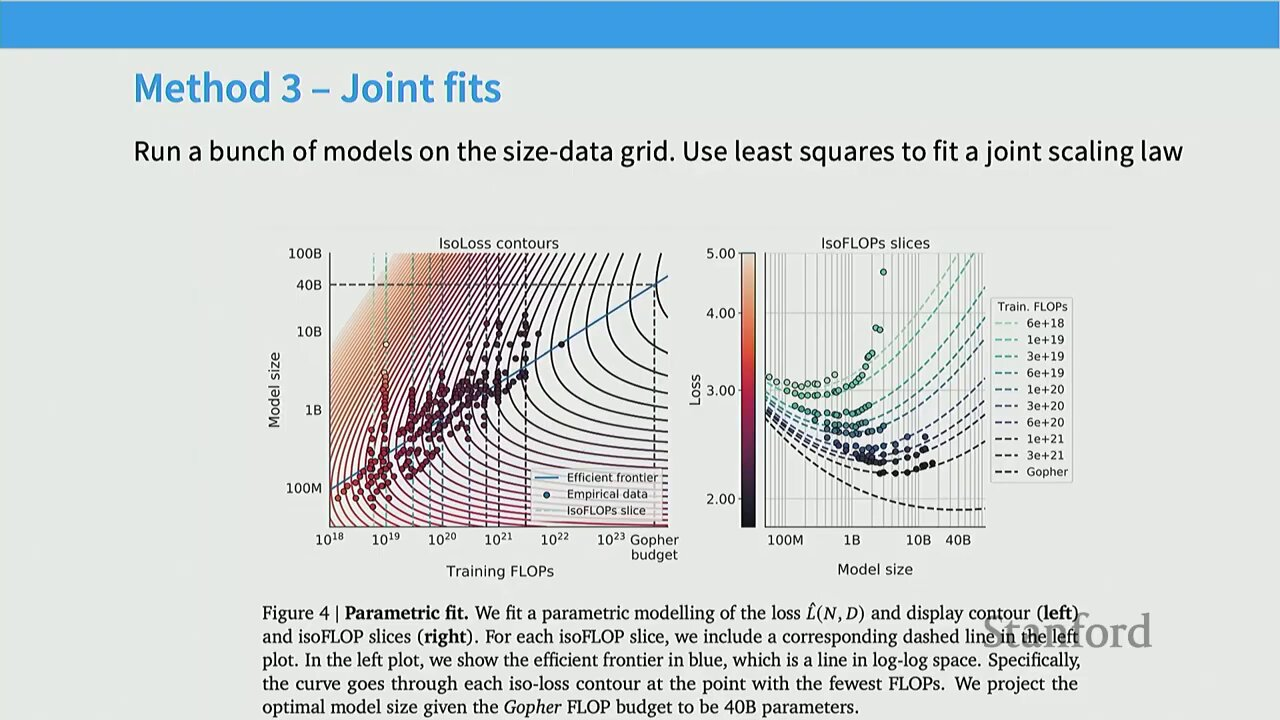
\includegraphics[width=0.92\textwidth]{figures/fig_chinchilla_method3.jpg}
\caption{Chinchilla Method 3：直接拟合 Rosenfeld 形式 $L(N,D) = \alpha + \beta/N^p + \gamma/D^q$ 到所有数据点。原始拟合残差有非零均值导致偏差，Epoch AI 复现修正后与 Method 1/2 一致。\protect\footnotemark}
\end{figure}
\footnotetext{视频画面时间区间：00:58:45--00:59:15。}

Method 3 直接拟合联合 loss 模型 $L(N,D) = \alpha + \beta N^{-p} + \gamma D^{-q}$，再用拉格朗日法在约束 $C \approx 6ND$ 下求最优 $(N^{\*}, D^{\*})$。

\begin{warningbox}{原始 Method 3 的拟合偏差}
Percy 指出：Chinchilla 原始 Method 3 的拟合残差存在\textbf{非零均值}，意味着模型对中等规模点存在系统偏差。这个偏差被\textbf{Epoch AI 的独立复现}修正后，给出的最优 $(N^{\*}, D^{\*})$ 与 Method 1、Method 2 高度一致。\textbf{三方法殊途同归}，是 Chinchilla 结论稳健性的最强背书。
\end{warningbox}

\subsection{核心结论：20 tokens / parameter}

三种方法都收敛到同一结论：\textbf{在 compute-optimal 点}，数据与参数的比例约为
\[
\frac{D^{\*}}{N^{\*}} \;\approx\; 20.
\]
即每个参数应配约 20 个训练 token。这与 Kaplan 的"GPT-3 约 2 tokens/parameter"形成鲜明对比。

\begin{importantbox}{Chinchilla 的工程冲击}
Chinchilla 之前，业界倾向"建更大的模型、用更少的数据"；Chinchilla 之后，趋势反转：\textbf{同等 compute 下，更小的模型 + 更多的数据更划算}。这直接催生了 Llama 系列等"小而精"的开放模型路线。
\end{importantbox}

\section{Tokens-per-parameter 的演化}

\begin{figure}[H]
\centering
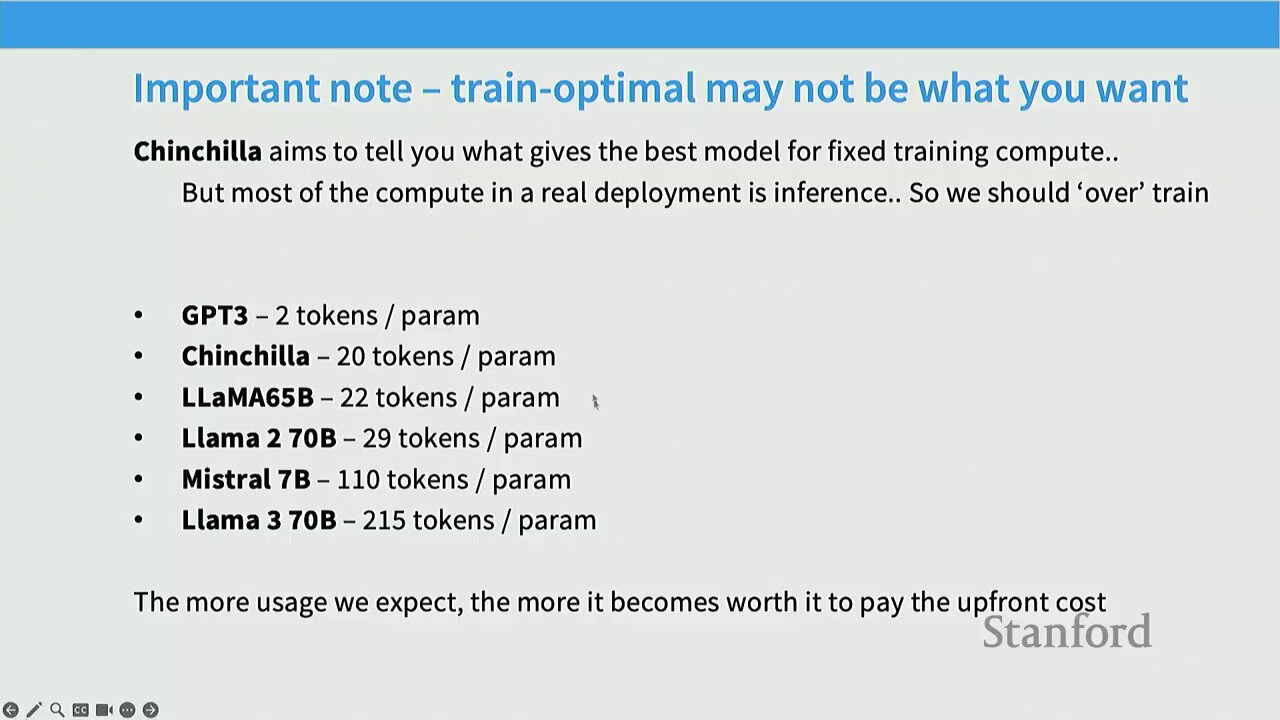
\includegraphics[width=0.92\textwidth]{figures/fig_tokens_per_param_evolution.jpg}
\caption{Tokens/parameter 比随时间的演化：GPT-3 约 2 $\to$ Chinchilla 20 $\to$ 现代（Llama、Qwen 等）远超 20，因推理成本主导而倾向"over-train 小模型"。\protect\footnotemark}
\end{figure}
\footnotetext{视频画面时间区间：01:01:45--01:02:15。}

\begin{knowledgebox}{从 20 到远超 20：推理经济学}
Percy 在课末点出一个当代演化：Chinchilla 给出 compute-optimal 比是 20，但工业界很快就\textbf{主动超过这个值}。原因在于\textbf{推理经济学}：
\[
\text{总成本} \;=\; \underbrace{\text{训练成本（一次性）}}_{\text{愿多付}} \;+\; \underbrace{\text{推理成本（持续、海量）}}_{\text{要省}}.
\]
推理成本与参数量成正比，因此\textbf{宁愿在训练阶段 over-train 一个更小的模型}（用更多 token 换更小参数），让长期推理更便宜。例如最新 Qwen 系列报告在 30 trillion tokens 上训练，tokens/parameter 远超 20。
\end{knowledgebox}

这告诉我们：\textbf{Chinchilla 的 20 不是"正确答案"，而是"训练- compute- 最优"的答案}。一旦把推理成本纳入考量，最优 ratio 会向更大的数据-参数比漂移。

\section{Scaling law 的可复现性：扩散模型的旁证}

Percy 在课末分享了一个有趣的旁证：他的学生 Isan 在研究\textbf{扩散模型用于文本生成}时，面对一个全新类型的生成模型——既不知道最优 token/parameter 比，也不知道它"是否"会 scale。\textbf{把 IsoFLOP 分析的同一套 playbook 拿过来直接跑，得到了几乎与自回归模型一致的 Chinchilla 式曲线}，两者只差一个常数偏移。

\begin{importantbox}{Scaling law 不是 cherry-picked}
这个案例说明：\textbf{scaling law 不是自回归模型独有的、被精心挑选的现象}。它在完全不同的生成机制（扩散 vs 自回归）上自然复现。这是对 scaling law 作为"通用经验规律"地位的有力背书。
\end{importantbox}

\section{总结与延伸}

\begin{figure}[H]
\centering
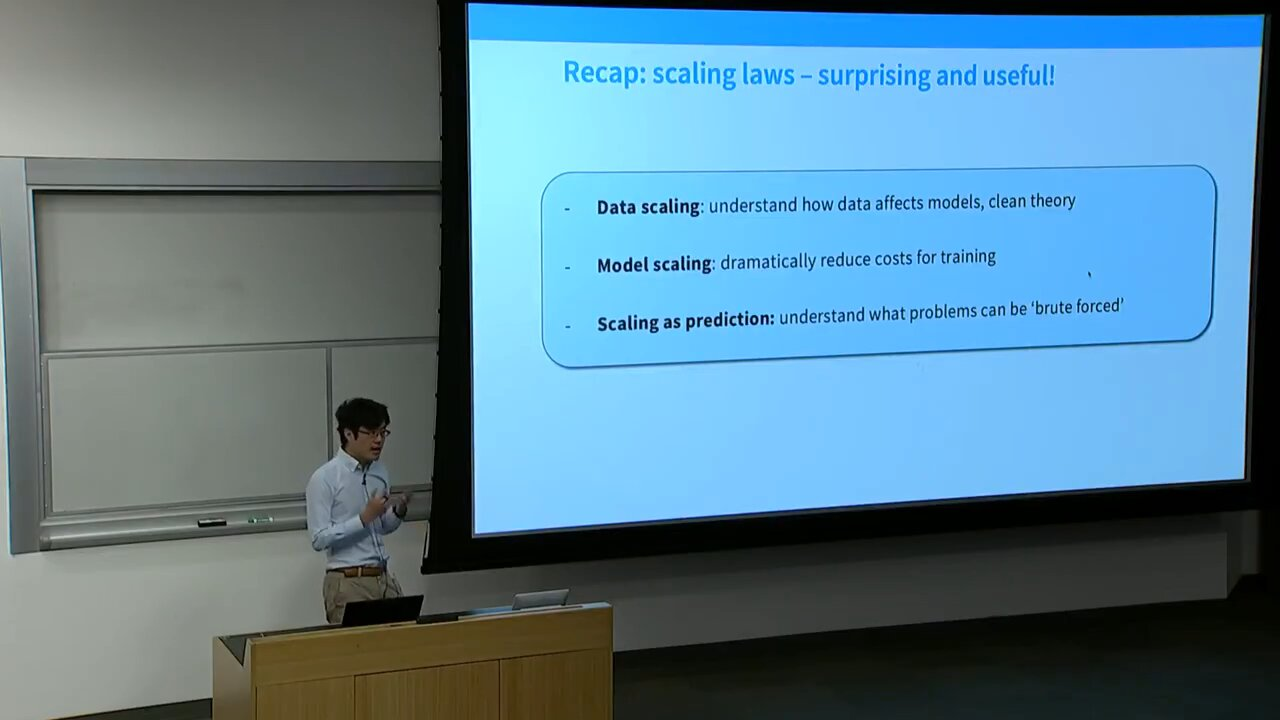
\includegraphics[width=0.92\textwidth]{figures/fig_summary.jpg}
\caption{全讲总结：log-log 线性关系从数据维度扩展到模型参数与总 compute；支撑超参决策与 compute-data 资源权衡。\protect\footnotemark}
\end{figure}
\footnotetext{视频画面时间区间：01:04:45--01:05:15。}

\subsection{核心论点}

\begin{importantbox}{五个核心论点}
\begin{enumerate}
\item \textbf{幂律是普遍现象}：从 Bell Labs 1993 到 Chinchilla 2022，跨越三十多年和多个 ML 子领域反复出现。理论（均值估计、非参数回归）只能解释"为什么是幂律"，但解释不了实测指数。
\item \textbf{实测指数远比理论慢}：MT $\approx 0.13$、speech $\approx 0.3$、LM $\approx 0.95$，远小于 PAC 界的 $0.5$，反映真实任务的高内在维度。
\item \textbf{架构与优化器改变常数、不改变指数}：这让"小规模实验比较效率、再迁移到大规模"成为可行工程范式（hyperparameter transfer）。
\item \textbf{Kaplan 偏差源于实验设计}（尤其是 cosine LR schedule 的截断问题），导致 GPT-3 时代"参数过多、数据过少"的系统性偏差。
\item \textbf{Chinchilla 三方法殊途同归}给出 compute-optimal ratio $\approx 20$ tokens/parameter；但加入推理经济学后，工业界主动超过这个值。
\end{enumerate}
\end{importantbox}

\subsection{关键公式速查}

\begin{tabular}{p{6cm}p{7cm}}
\toprule
\textbf{公式} & \textbf{含义} \\
\midrule
$L(m)=\alpha+\beta\,m^{-p}$ & Bell Labs 单变量幂律：$\alpha$ 不可约误差，$p$ 衰减指数 \\
$\mathrm{Var}(\bar{x})=\sigma^2/n$ & 均值估计的理论 scaling（$p=1$） \\
$\text{MSE}\sim n^{-2/(d+1)}$ & 非参数回归：指数由内在维度 $d$ 决定 \\
$L(N,D)=\alpha+\beta/N^p+\gamma/D^q$ & Rosenfeld / Chinchilla 联合曲面 \\
$D^{\*}/N^{\*}\approx 20$ & Chinchilla compute-optimal 比例 \\
$C\approx 6ND$ & Transformer 训练 FLOPs 近似公式 \\
\bottomrule
\end{tabular}

\subsection{配套阅读}

以下论文建议按本讲内容对照阅读：

\begin{tabular}{p{7cm}p{6cm}}
\toprule
\textbf{论文} & \textbf{对应知识点} \\
\midrule
Kaplan et al.\ 2020《Scaling Laws for Neural LM》 & 单变量幂律、aspect ratio、non-embedding $N$ \\
Hoffmann et al.\ 2022《Chinchilla》 & 三方法、20 tokens/parameter \\
Hestness et al.\ 2017《Deep Learning Scaling is Predictable》 & 三区域、跨任务指数 \\
Rosenfeld et al.\ 2019/2020 & 联合曲面 $L(N,D)=\alpha+\beta/N^p+\gamma/D^q$ \\
Banko \& Brill 2001 & "more data beats cleverer algorithms" \\
Yang et al.\ 《Tensor Programs V：muP》 & 学习率的 hyperparameter transfer \\
McCandlish et al.\ 2018《Natural Noise Scale》 & Critical batch size 理论 \\
\bottomrule
\end{tabular}

\subsection{下节预告}

下一讲（Scaling Laws 2）将进一步讨论：\textbf{超越 Chinchilla 的现代 scaling law}（如 Llama 3 训练报告中的实测曲线）、\textbf{breaking scaling laws}（如何通过架构/数据质量改进来"打破"既有幂律）、以及\textbf{scaling law 在 RLHF / 后训练阶段}的适用性。

%% --- 正文内容结束 ---

\end{document}
